%
\begin{isabellebody}%
\def\isabellecontext{AbstractObjects}%
%
\isadelimtheory
%
\endisadelimtheory
%
\isatagtheory
%
\endisatagtheory
{\isafoldtheory}%
%
\isadelimtheory
%
\endisadelimtheory
%
\begin{isamarkuptext}%
\begin{abstract}
We present an attempt to formalize modal relational type theory in functional type theory. This
formalization has been motivated to serve as a possible starting point for the subsequent modeling
of Zalta's theory of abstract objects, which  provides an axiomatic foundation for metaphysics.
\end{abstract}%
\end{isamarkuptext}%
\isamarkuptrue%
%
\isamarkupsection{Introduction%
}
\isamarkuptrue%
%
\begin{isamarkuptext}%
The principia metaphysica project\footnote{Cf.~\url{https://mally.stanford.edu/principia/principia.html}} 
  \cite{zalta:_princ_metap} at Stanford University aims
  at providing an encompassing axiomatic foundation for metaphysics, mathematics and the sciences. 
  The starting point is Zalta's theory of abstract objects \cite{zalta83:_abstr_objec}  --- a metaphysical 
  theory providing a systematic description of fundamental and complex abstract objects. This 
  theory provides is at heart of Zalta's ongoing 'principia metaphysica' 
  project.
  
  The theory of abstract objects utilizes a modal relational type theory (MRTT) as 
  logical foundation.  Arguments
  defending this choice against a modal functional type theory (MFTT)
  have been presented before \cite{zalta11:_relat_versus_funct_found_logic}.
  In a nutshell, the situation is this: functional type theory comes with strong 
  comprehension principles, which, in the context of the theory of abstract objects, 
  have paradoxical implications \cite[chap.4]{zalta11:_relat_versus_funct_found_logic}. 
  When starting off with a relational foundation, however, 
  weaker comprehension principles are provided, and these obstacles can be avoided.

  Isabelle/HOL is a proof assistant based on a functional type theory extending
  Church's theory of types \cite{Church40}, and recently it has been shown 
  that Church's type theory can be elegantly utilized as a meta-logic to semantically embed and 
  automate various quantified non-classical logics, including MFTT \cite{J23,C40}. 
  This embedding of MFTT has subsequently been employed in a case study in
  computational metaphysics, in which different variants of Kurt G{\"o}del's ontological 
  argument were verified resp. falsified \cite{C40,C55}. 

  In this paper we explore an idea to encode, respectively embed,  MRTT in functional type theory. 
  Thereby, we want adapt and extend ideas from the previous, successful embedding of MFTT in functional 
  type theory.
  Our contribution here shall serve as possible starting point for the subsequent
  formalization of further chapters of the theory of abstract objects and the principia 
  metaphysica -- as far as this is possible considering the technical challenges we report below. 

 
  The motivating research questions for the formalisation presented below include:
  \begin{itemize} 
  \item Can functional type theory, despite the problems as pointed 
   out by Zalta and
   Oppenheimer \cite{zalta11:_relat_versus_funct_found_logic}, 
   nevertheless be utilized to encode MRTT and subsequently the theory of abstract 
   objects when adapting and utilizing the embeddings approach? 
   % As it turns, we will 
   % need a significant, technically involved extension of the embeddings approach.
  \item From another perspective we are interested in studying options to restrict comprehension in 
   functional type theory when utilizing the embedding approach.
  \item From a pragmatic point of view, we want to assess the user-friendliness of 
   the proposed solution? 
   To what extend can Isabelle's  user interface hide 
   unpleasant technicalities of the extended embedding from the user?
  \item How far can automation be pushed in the approach? For this note that proof automation 
    worked  well for the simpler embeddings as utilized in previous work \cite{C40,C55}. 
  %\item Can the consistency of the theory eventually be validated with the available automated 
  % reasoning tools?
  %\item Can the reasoners eventually even contribute some new knowledge? 
  %\item Are any suggestions  arising for possible improvements in Isabelle/HOL.
  % What are the particular problems detected in the course of the study?
  \end{itemize}

  In this paper we focus mainly on the presentation of the embedding of MRTT in functional type theory.
  Some technical difficulties will be highlighted. However, a proper exploration and discussion of 
  the above questions is left as further work.
 


  The formalization idea we explore below is to adapt and extend the previous encoding of MFTT in 
  functional type theory. 
  The basic idea of this encoding is simple: modal logic formulas are identified with certain functional 
  type theory formulas of predicate type \isa{i{\isasymRightarrow}bool} (abbreviated as \isa{io} below). 
  Possible worlds are explicitly represented as
  terms of type  \isa{i}. A modal logic formula \isa{{\isasymphi}} holds for a world \isa{w} if and 
  only if the application \isa{{\isacharparenleft}{\isasymphi}\ w{\isacharparenright}} evaluates to true. The definitions of the propositional modal logic 
  connectives are straightforward. These definitions realize the well known standard translation as a set of equations 
  in functional type theory and they successfully extend the standard translation also for quantifiers. An important
  aspect thereby is that quantifiers can be handled just as ordinary logical connectives. No binding mechanisms are needed,
  since the binding mechanism for lambda-abstractions can be fruitfully utilised.
  
  The challenge for the work presented here has been to suitably 'restrict' this embedding for MRTT (instead of MFTT).
  However, as we will see, this restriction is achieved below by introducing a technically involved 
  additional layer in the embedding; this additional layer provides means to annotate formulas and terms with
  grammatical information.
 
  The grammar of the second-order fragment of MRTT is presented in Figure~\ref{mmrt}; detailed descriptions
  of MRTT are available in the literature (see e.g. the appendix of \cite{Zalta88}).
 
   \begin{figure}[t]
  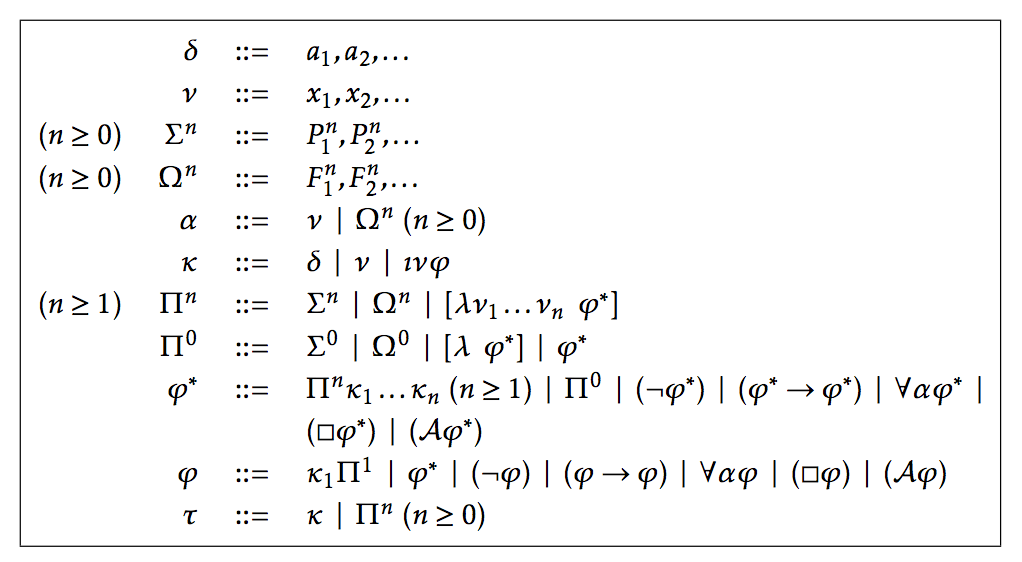
\includegraphics[height=5.5cm]{ModalRelationalTypeTheory.png}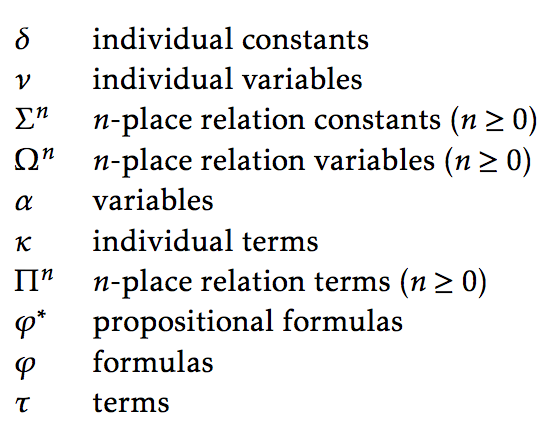
\includegraphics[height=4.5cm]{ModalRelationalTypeTheory2.png}
  \caption{Grammar of MRTT, cf. \cite{zalta:_princ_metap} for further details. \label{mmrt}
  Two kinds of (complex) formulas are introduced: the $\varphi$-formulas may have encoding subformulas, while the
  $\varphi^*$-formulas must not. The latter are designated as propositional formulas, the former ones simply as formulas.}
  \end{figure}
  Note that this grammar successfully excludes terms such as $(\lambda x \exists F. xF \wedge \neg Fx)$, where $Fx$ represents 
  exemplification of property $F$ by $x$ and $xF$ stands for the encoding of property $F$ by $x$. It are such kind of  
  lambda-abstractions which lead to paradoxical situations in the theory of abstract 
  objects \cite[chap.4]{zalta11:_relat_versus_funct_found_logic}.
  

  To achieve our goal we provide means to explicitly represent, maintain and propagate information  on the 
  syntactical structure of MRTT in functional type theory. In particular, we provide means in form of annotations 
  to explicitly distinguish 
  between propositional formulas, formulas, terms and erroneous (ineligible/excluded) formations. 
  Respective annotation information is propagated from the innermost constituents to the top level constructions.
  This creates some non-trivial technical overhead. However, due to Isabelle/HOL's user 
  interface these technicalities can be hidden from the user (to some extend). 

  A note on using abbreviations versus definitions in our approach:  We are aware that abbreviations should
  be used sparsingly in Isabelle/HOL; they are automatically expanded and thus lead to a discrepancy 
  between the internal and the external view of a term. However, we here deliberately deviate from this
  rule, since one aspect of the paper is to particularly illustrate exactly this discrepancy and to emphasize the complexity
  of the embedding MRTT in functional type theory.\footnote{We have also 
  experimented with using definitions instead of abbreviations; respective 
  encoding fragments can be requested from the first author.} 

  In fact, as we believe, the technical  complexity of the embedding presented below  pen and paper 
  work with it pragmatically infeasible. In this sense, we agree with previous 
  findings \cite{zalta11:_relat_versus_funct_found_logic}. 

  On the other hand, we illustrate the feasibility of maintaining and propagating 
  grammatical information in connection with a shallow
  embedding approach. Remember, that one central aim has been to suitably
  restrict the comprehension principles for the embedded MRTT despite the fact that underlying functional 
  type theory comes with full comprehension principles.  
 
  Our hope has been that the proposed approach can eventually be pragmatically handled to 
  at least some modest degree in a modern proof assistant such as Isabelle/HOL. In fact, as we will also
  illustrate, the simplifier \isa{simp} of Isabelle is indeed well capable of effectively reducing
  the technically inflated terms we obtain from the extended embedding to its logical core content.  
  In other words, Isabelle's simplifier effectievely analyses and and rewrites the 
  deeply annotated terms and propagates the annotation information as intended to top-level.
  It thus seems feasable, to some degree, to seperate the rasoning about annotations from 
  the reasoning about logical content within our shallow embedding approach.%
\end{isamarkuptext}%
\isamarkuptrue%
%
\isamarkupsection{Preliminaries%
}
\isamarkuptrue%
%
\begin{isamarkuptext}%
We start out with some type declarations and type abbreviations. 
  Remember that our formalism explicitly encodes possible world semantics. Hence, we introduce a 
  distinguished type \isa{i} to represent the set of possible worlds. 
  Consequently, terms of this type denote possible worlds. 
  Moreover, modal logic formulas are associated in our approach with
  predicates on (resp. sets of) on possible worlds. Hence, modal logic formulas have
  type \isa{{\isacharparenleft}i\ {\isasymRightarrow}\ bool{\isacharparenright}}. To make our representation  more concise in the remainder
  we abbreviate this type as \isa{io}.%
\end{isamarkuptext}%
\isamarkuptrue%
\ \isacommand{typedecl}\isamarkupfalse%
\ i\ \isanewline
\ \isacommand{type{\isacharunderscore}synonym}\isamarkupfalse%
\ io\ {\isacharequal}\ {\isachardoublequoteopen}{\isacharparenleft}i{\isasymRightarrow}bool{\isacharparenright}{\isachardoublequoteclose}%
\begin{isamarkuptext}%
Entities in the abstract theory of types are represented in our formalism by the
  type \isa{e}. We call this the raw type of entities resp. objects. The Theory of Abstract Objects 
  later introduces means to distinguish between abstract and ordinary entities.%
\end{isamarkuptext}%
\isamarkuptrue%
\ \isacommand{typedecl}\isamarkupfalse%
\ e%
\begin{isamarkuptext}%
To explicitly model the syntactical restrictions of MRTT we introduce a 
  (polymorphic) datatype \isa{{\isacharprime}a\ opt} (\isa{{\isacharprime}a} is a type variable) 
  based on four constructors: \isa{ERR\ {\isacharprime}a} (identifies ineligible/excluded constructions), \isa{P\ {\isacharprime}a} 
  (identifies propositional formulas), \isa{F\ {\isacharprime}a} (identifies  formulas), and \isa{T\ {\isacharprime}a} (identifies 
  eligible terms, such as constants and lambda abstractions). The embedding approach (of MFTT in functional type theory)
  is suitably adapted below so that 
  for each language expression (in the embedded MRTT) the respective datatype 
  is identified and appropriately propagated. The encapsulated expressions  
  correspond to the previous embedding of MRTT in functional type theory  \cite{J23,C40}.%
\end{isamarkuptext}%
\isamarkuptrue%
\ \isacommand{datatype}\isamarkupfalse%
\ {\isacharprime}a\ opt\ {\isacharequal}\ ERR\ {\isacharprime}a\ {\isacharbar}\ P\ {\isacharprime}a\ {\isacharbar}\ F\ {\isacharprime}a\ {\isacharbar}\ T\ {\isacharprime}a%
\begin{isamarkuptext}%
The following operators support a concise and elegant superscript annotation with these
  four syntactical categories for our language constructs.%
\end{isamarkuptext}%
\isamarkuptrue%
\ \isacommand{abbreviation}\isamarkupfalse%
\ mkP{\isacharcolon}{\isacharcolon}{\isachardoublequoteopen}io{\isasymRightarrow}io\ opt{\isachardoublequoteclose}\ {\isacharparenleft}{\isachardoublequoteopen}{\isacharunderscore}\isactrlsup P{\isachardoublequoteclose}\ {\isacharbrackleft}{\isadigit{1}}{\isadigit{0}}{\isadigit{9}}{\isacharbrackright}\ {\isadigit{1}}{\isadigit{1}}{\isadigit{0}}{\isacharparenright}\ \ \isakeyword{where}\ {\isachardoublequoteopen}{\isasymphi}\isactrlsup P\ {\isasymequiv}\ P\ {\isasymphi}{\isachardoublequoteclose}\ \isanewline
\ \isacommand{abbreviation}\isamarkupfalse%
\ mkF{\isacharcolon}{\isacharcolon}{\isachardoublequoteopen}io{\isasymRightarrow}io\ opt{\isachardoublequoteclose}\ {\isacharparenleft}{\isachardoublequoteopen}{\isacharunderscore}\isactrlsup F{\isachardoublequoteclose}\ {\isacharbrackleft}{\isadigit{1}}{\isadigit{0}}{\isadigit{9}}{\isacharbrackright}\ {\isadigit{1}}{\isadigit{1}}{\isadigit{0}}{\isacharparenright}\ \ \isakeyword{where}\ {\isachardoublequoteopen}{\isasymphi}\isactrlsup F\ {\isasymequiv}\ F\ {\isasymphi}{\isachardoublequoteclose}\ \isanewline
\ \isacommand{abbreviation}\isamarkupfalse%
\ mkT{\isacharcolon}{\isacharcolon}{\isachardoublequoteopen}{\isacharprime}a{\isasymRightarrow}{\isacharprime}a\ opt{\isachardoublequoteclose}\ {\isacharparenleft}{\isachardoublequoteopen}{\isacharunderscore}\isactrlsup T{\isachardoublequoteclose}\ {\isacharbrackleft}{\isadigit{1}}{\isadigit{0}}{\isadigit{9}}{\isacharbrackright}\ {\isadigit{1}}{\isadigit{1}}{\isadigit{0}}{\isacharparenright}\ \ \isakeyword{where}\ {\isachardoublequoteopen}{\isasymphi}\isactrlsup T\ {\isasymequiv}\ T\ {\isasymphi}{\isachardoublequoteclose}\isanewline
\ \isacommand{abbreviation}\isamarkupfalse%
\ mkE{\isacharcolon}{\isacharcolon}{\isachardoublequoteopen}{\isacharprime}a{\isasymRightarrow}{\isacharprime}a\ opt{\isachardoublequoteclose}\ {\isacharparenleft}{\isachardoublequoteopen}{\isacharunderscore}\isactrlsup E{\isachardoublequoteclose}\ {\isacharbrackleft}{\isadigit{1}}{\isadigit{0}}{\isadigit{9}}{\isacharbrackright}\ {\isadigit{1}}{\isadigit{1}}{\isadigit{0}}{\isacharparenright}\ \ \isakeyword{where}\ {\isachardoublequoteopen}{\isasymphi}\isactrlsup E\ {\isasymequiv}\ ERR\ {\isasymphi}{\isachardoublequoteclose}%
\begin{isamarkuptext}%
Certain language constructs in the Theory of Abstract objects, such as the actuality operator  
  \isa{\isactrlbold {\isasymA}} ("it is actually the case that"), refer to a (fixed) designated world. To model such a 
  rigid dependence we introduce a constant symbol (name) \isa{dw} of world type \isa{i}. 
  Moreover, for technical reasons, 
  which will be clarified below, we introduce further (dummy) constant symbols for the various other domains. 
  We anyway assume that all domains are non-empty. Hence, introducing these constant symbols is obviously not 
  harmful.\footnote{The single polymorphic dummy \isa{da{\isacharcolon}{\isacharcolon}{\isacharprime}a}, utilized e.g. in the definition of the universal 
  quantifier of MRTT below, actually covers already all cases. However, to avoid unnecessary type inferences we
  actually prefer non-polymorphic dummy elements in all those cases where we can statically 
  determine the required type.}%
\end{isamarkuptext}%
\isamarkuptrue%
\ \isacommand{consts}\isamarkupfalse%
\ dw{\isacharcolon}{\isacharcolon}{\isachardoublequoteopen}i{\isachardoublequoteclose}\ \isanewline
\ \isacommand{consts}\isamarkupfalse%
\ de{\isacharcolon}{\isacharcolon}{\isachardoublequoteopen}e{\isachardoublequoteclose}\ dio{\isacharcolon}{\isacharcolon}{\isachardoublequoteopen}io{\isachardoublequoteclose}\ deio{\isacharcolon}{\isacharcolon}{\isachardoublequoteopen}e{\isasymRightarrow}io{\isachardoublequoteclose}\ da{\isacharcolon}{\isacharcolon}{\isachardoublequoteopen}{\isacharprime}a{\isachardoublequoteclose}%
\isamarkupsection{Embedding of Modal Relational Type Theory%
}
\isamarkuptrue%
%
\begin{isamarkuptext}%
The various language constructs of MRTT (see Figure \ref{mmrt}) are now introduced step by step.%
\end{isamarkuptext}%
\isamarkuptrue%
%
\begin{isamarkuptext}%
The actuality operator \isa{\isactrlbold {\isasymA}}, when being applied to a formula or propositional formula 
  \isa{{\isasymphi}}, evaluates \isa{{\isasymphi}} wrt the fixed given world \isa{dw}. 
  The compound expression \isa{\isactrlbold {\isasymA}{\isasymphi}} inherits its syntactical category  \isa{F} (formula) or
  \isa{P} (propositional formula) from \isa{{\isasymphi}}. If the syntactical category of  \isa{{\isasymphi}} is 
  \isa{ERR} (error) or \isa{T} (term), then the syntactical category of \isa{\isactrlbold {\isasymA}{\isasymphi}} 
  is \isa{ERR} and a dummy entity of appropriate type is returned. This illustrates the core 
  ideas of our explicit modeling of MRTT grammatical structure in functional type theory. 
  This scheme will repeated below for all the other language constructs of MRTT.%
\end{isamarkuptext}%
\isamarkuptrue%
\ \isacommand{abbreviation}\isamarkupfalse%
\ Actual{\isacharcolon}{\isacharcolon}{\isachardoublequoteopen}io\ opt\ {\isasymRightarrow}\ io\ opt{\isachardoublequoteclose}\ {\isacharparenleft}{\isachardoublequoteopen}\isactrlbold {\isasymA}\ {\isacharunderscore}{\isachardoublequoteclose}\ {\isacharbrackleft}{\isadigit{6}}{\isadigit{4}}{\isacharbrackright}\ {\isadigit{6}}{\isadigit{5}}{\isacharparenright}\ \isakeyword{where}\ {\isachardoublequoteopen}\isactrlbold {\isasymA}{\isasymphi}\ {\isasymequiv}\ case\ {\isasymphi}\ of\ \isanewline
\ \ \ \ F{\isacharparenleft}{\isasympsi}{\isacharparenright}\ {\isasymRightarrow}\ F{\isacharparenleft}{\isasymlambda}w{\isachardot}\ {\isasympsi}\ dw{\isacharparenright}\ {\isacharbar}\ \isanewline
\ \ \ \ P{\isacharparenleft}{\isasympsi}{\isacharparenright}\ {\isasymRightarrow}\ P{\isacharparenleft}{\isasymlambda}w{\isachardot}\ {\isasympsi}\ dw{\isacharparenright}\ {\isacharbar}\ \isanewline
\ \ \ \ {\isacharunderscore}\ {\isasymRightarrow}\ ERR{\isacharparenleft}dio{\isacharparenright}{\isachardoublequoteclose}%
\begin{isamarkuptext}%
The Theory of Abstract Objects distinguishes between encoding properties \isa{{\isasymkappa}\isactrlsub {\isadigit{1}}{\isasymPi}\isactrlsup {\isadigit{1}}} and 
  exemplifying properties \isa{{\isasymPi}\isactrlsup n{\isacharcomma}{\isasymkappa}\isactrlsub {\isadigit{1}}{\isacharcomma}{\isachardot}{\isachardot}{\isacharcomma}{\isasymkappa}\isactrlsub n} (for $n\geq 1$). 

  Encoding \isa{{\isasymkappa}{\isasymPi}} is noted below as \isa{{\isasymlbrace}{\isasymkappa}{\isacharcomma}{\isasymPi}{\isasymrbrace}}.
  Encoding yields formulas and never propositional formulas and it is mapped below
  to predicate application \isa{{\isasymPi}{\isacharparenleft}{\isasymkappa}{\isacharparenright}}. This way we inherit the lambda conversion principles for 
  encoding from the underlying meta-logic.
  Exemplification is be noted below as \isa{{\isasymlparr}{\isasymPi}{\isacharcomma}x{\isasymrparr}} (respectively, \isa{{\isasymlparr}{\isasymPi}{\isacharcomma}x{\isacharcomma}{\isachardot}{\isachardot}{\isachardot}{\isasymrparr}}).
  It is mapped to expressions of 
  form \isa{{\isacharparenleft}exe\ {\isasymPi}{\isacharparenleft}{\isasymkappa}{\isacharparenright}}, where \isa{exe} is uninterpreted constant symbol of appropriate 
  type. Again, lambda conversion principles are inherited 
  from the underlying meta-logic, but only 'under the hood' of the guarding \isa{exe}-predicate.
  We do not map both, encoding and exemplification, to unguarded predicate application in the meta-logic, since this
  would conflate both notions and allow us to prove statements such as \isa{{\isasymlbrace}{\isasymkappa}{\isacharcomma}{\isasymPi}{\isasymrbrace}\ \isactrlbold {\isasymrightarrow}\ {\isasymlparr}{\isasymPi}{\isacharcomma}x{\isasymrparr}}.%
\end{isamarkuptext}%
\isamarkuptrue%
\ \isacommand{consts}\isamarkupfalse%
\ enc{\isacharcolon}{\isacharcolon}{\isachardoublequoteopen}io{\isasymRightarrow}io{\isachardoublequoteclose}\isanewline
\ \isacommand{abbreviation}\isamarkupfalse%
\ Enc{\isacharcolon}{\isacharcolon}{\isachardoublequoteopen}e\ opt{\isasymRightarrow}{\isacharparenleft}e{\isasymRightarrow}io{\isacharparenright}\ opt{\isasymRightarrow}io\ opt{\isachardoublequoteclose}\ {\isacharparenleft}{\isachardoublequoteopen}{\isasymlbrace}{\isacharunderscore}{\isacharcomma}{\isacharunderscore}{\isasymrbrace}{\isachardoublequoteclose}{\isacharparenright}\ \isakeyword{where}\ {\isachardoublequoteopen}{\isasymlbrace}x{\isacharcomma}{\isasymPhi}{\isasymrbrace}\ {\isasymequiv}\ case\ {\isacharparenleft}x{\isacharcomma}{\isasymPhi}{\isacharparenright}\ of\ \isanewline
\ \ \ \ {\isacharparenleft}T{\isacharparenleft}y{\isacharparenright}{\isacharcomma}T{\isacharparenleft}Q{\isacharparenright}{\isacharparenright}\ {\isasymRightarrow}\ F{\isacharparenleft}Q\ y{\isacharparenright}\ {\isacharbar}\ \isanewline
\ \ \ \ {\isacharunderscore}\ {\isasymRightarrow}\ ERR{\isacharparenleft}dio{\isacharparenright}{\isachardoublequoteclose}%
\begin{isamarkuptext}%
Unary exemplifying formulas \isa{{\isasymPi}{\isasymkappa}} are noted as \isa{{\isasymlparr}{\isasymPi}{\isacharcomma}{\isasymkappa}{\isasymrparr}}.  
  Exemplification yields propositional formulas. 
  It is mapped to guarded predicate application; the guard is an uninterpreted predicate constant
  \isa{exe}.%
\end{isamarkuptext}%
\isamarkuptrue%
\ \isacommand{consts}\isamarkupfalse%
\ exe{\isacharcolon}{\isacharcolon}{\isachardoublequoteopen}io{\isasymRightarrow}io{\isachardoublequoteclose}\isanewline
\ \isacommand{abbreviation}\isamarkupfalse%
\ Exe{\isadigit{1}}{\isacharcolon}{\isacharcolon}{\isachardoublequoteopen}{\isacharparenleft}e{\isasymRightarrow}io{\isacharparenright}\ opt{\isasymRightarrow}e\ opt{\isasymRightarrow}io\ opt{\isachardoublequoteclose}\ {\isacharparenleft}{\isachardoublequoteopen}{\isasymlparr}{\isacharunderscore}{\isacharcomma}{\isacharunderscore}{\isasymrparr}{\isachardoublequoteclose}{\isacharparenright}\ \isakeyword{where}\ {\isachardoublequoteopen}{\isasymlparr}{\isasymPhi}{\isacharcomma}x{\isasymrparr}\ {\isasymequiv}\ case\ {\isacharparenleft}{\isasymPhi}{\isacharcomma}x{\isacharparenright}\ of\ \isanewline
\ \ \ \ {\isacharparenleft}T{\isacharparenleft}Q{\isacharparenright}{\isacharcomma}T{\isacharparenleft}y{\isacharparenright}{\isacharparenright}\ {\isasymRightarrow}\ P{\isacharparenleft}exe\ {\isacharparenleft}Q\ y{\isacharparenright}{\isacharparenright}\ {\isacharbar}\ \isanewline
\ \ \ \ {\isacharunderscore}\ {\isasymRightarrow}\ ERR{\isacharparenleft}dio{\isacharparenright}{\isachardoublequoteclose}%
\begin{isamarkuptext}%
For pragmatical reasons we support n-ary exemplification formulas \isa{{\isasymPi}\isactrlsup n{\isacharcomma}{\isasymkappa}\isactrlsub {\isadigit{1}}{\isacharcomma}{\isachardot}{\isachardot}{\isacharcomma}{\isasymkappa}\isactrlsub n} here only for \isa{{\isadigit{1}}{\isasymle}n{\isasymle}{\isadigit{3}}}.
 In addition to the unary case above, we thus introduce two further cases.%
\end{isamarkuptext}%
\isamarkuptrue%
\ \isacommand{abbreviation}\isamarkupfalse%
\ Exe{\isadigit{2}}{\isacharcolon}{\isacharcolon}{\isachardoublequoteopen}{\isacharparenleft}e{\isasymRightarrow}e{\isasymRightarrow}io{\isacharparenright}\ opt{\isasymRightarrow}e\ opt{\isasymRightarrow}e\ opt{\isasymRightarrow}io\ opt{\isachardoublequoteclose}\ {\isacharparenleft}{\isachardoublequoteopen}{\isasymlparr}{\isacharunderscore}{\isacharcomma}{\isacharunderscore}{\isacharcomma}{\isacharunderscore}{\isasymrparr}{\isachardoublequoteclose}{\isacharparenright}\isanewline
\ \ \isakeyword{where}\ {\isachardoublequoteopen}{\isasymlparr}{\isasymPhi}{\isacharcomma}x{\isadigit{1}}{\isacharcomma}x{\isadigit{2}}{\isasymrparr}\ {\isasymequiv}\ case\ {\isacharparenleft}{\isasymPhi}{\isacharcomma}x{\isadigit{1}}{\isacharcomma}x{\isadigit{2}}{\isacharparenright}\ of\ \isanewline
\ \ \ \ {\isacharparenleft}T{\isacharparenleft}Q{\isacharparenright}{\isacharcomma}T{\isacharparenleft}y{\isadigit{1}}{\isacharparenright}{\isacharcomma}T{\isacharparenleft}y{\isadigit{2}}{\isacharparenright}{\isacharparenright}\ {\isasymRightarrow}\ P{\isacharparenleft}exe\ {\isacharparenleft}Q\ y{\isadigit{1}}\ y{\isadigit{2}}{\isacharparenright}{\isacharparenright}\ {\isacharbar}\ \isanewline
\ \ \ \ {\isacharunderscore}\ {\isasymRightarrow}\ ERR{\isacharparenleft}dio{\isacharparenright}{\isachardoublequoteclose}\isanewline
\ \isacommand{abbreviation}\isamarkupfalse%
\ Exe{\isadigit{3}}{\isacharcolon}{\isacharcolon}{\isachardoublequoteopen}{\isacharparenleft}e{\isasymRightarrow}e{\isasymRightarrow}e{\isasymRightarrow}io{\isacharparenright}\ opt{\isasymRightarrow}e\ opt{\isasymRightarrow}e\ opt{\isasymRightarrow}e\ opt{\isasymRightarrow}io\ opt{\isachardoublequoteclose}\ {\isacharparenleft}{\isachardoublequoteopen}{\isasymlparr}{\isacharunderscore}{\isacharcomma}{\isacharunderscore}{\isacharcomma}{\isacharunderscore}{\isacharcomma}{\isacharunderscore}{\isasymrparr}{\isachardoublequoteclose}{\isacharparenright}\ \isanewline
\ \ \isakeyword{where}\ {\isachardoublequoteopen}{\isasymlparr}{\isasymPhi}{\isacharcomma}x{\isadigit{1}}{\isacharcomma}x{\isadigit{2}}{\isacharcomma}x{\isadigit{3}}{\isasymrparr}\ {\isasymequiv}\ case\ {\isacharparenleft}{\isasymPhi}{\isacharcomma}x{\isadigit{1}}{\isacharcomma}x{\isadigit{2}}{\isacharcomma}x{\isadigit{3}}{\isacharparenright}\ of\ \isanewline
\ \ \ \ {\isacharparenleft}T{\isacharparenleft}Q{\isacharparenright}{\isacharcomma}T{\isacharparenleft}y{\isadigit{1}}{\isacharparenright}{\isacharcomma}T{\isacharparenleft}y{\isadigit{2}}{\isacharparenright}{\isacharcomma}T{\isacharparenleft}y{\isadigit{3}}{\isacharparenright}{\isacharparenright}\ {\isasymRightarrow}\ P{\isacharparenleft}exe\ {\isacharparenleft}Q\ y{\isadigit{1}}\ y{\isadigit{2}}\ y{\isadigit{3}}{\isacharparenright}{\isacharparenright}\ {\isacharbar}\ \isanewline
\ \ \ \ {\isacharunderscore}\ {\isasymRightarrow}\ ERR{\isacharparenleft}dio{\isacharparenright}{\isachardoublequoteclose}%
\begin{isamarkuptext}%
Formations with negation and implication are supported for both, formulas and propositional
  formulas, and their embeddings are straightforward. In the case of implication, the compound formula
  is a propositional formula if both constituents are propositional formulas. If at least one constituent 
  is a formula and the other one eligible, then the compound formula is a formula. In all other
  cases an ERR-Formula is returned.%
\end{isamarkuptext}%
\isamarkuptrue%
\ \isacommand{abbreviation}\isamarkupfalse%
\ not{\isacharcolon}{\isacharcolon}{\isachardoublequoteopen}io\ opt{\isasymRightarrow}io\ opt{\isachardoublequoteclose}\ {\isacharparenleft}{\isachardoublequoteopen}\isactrlbold {\isasymnot}\ {\isacharunderscore}{\isachardoublequoteclose}\ {\isacharbrackleft}{\isadigit{5}}{\isadigit{8}}{\isacharbrackright}\ {\isadigit{5}}{\isadigit{9}}{\isacharparenright}\ \isakeyword{where}\ {\isachardoublequoteopen}\isactrlbold {\isasymnot}\ {\isasymphi}\ {\isasymequiv}\ case\ {\isasymphi}\ of\ \isanewline
\ \ \ \ F{\isacharparenleft}{\isasympsi}{\isacharparenright}\ {\isasymRightarrow}\ F{\isacharparenleft}{\isasymlambda}w{\isachardot}{\isasymnot}{\isacharparenleft}{\isasympsi}\ w{\isacharparenright}{\isacharparenright}\ {\isacharbar}\ \isanewline
\ \ \ \ P{\isacharparenleft}{\isasympsi}{\isacharparenright}\ {\isasymRightarrow}\ P{\isacharparenleft}{\isasymlambda}w{\isachardot}{\isasymnot}{\isacharparenleft}{\isasympsi}\ w{\isacharparenright}{\isacharparenright}\ {\isacharbar}\ \isanewline
\ \ \ \ {\isacharunderscore}\ {\isasymRightarrow}\ ERR{\isacharparenleft}dio{\isacharparenright}{\isachardoublequoteclose}\ \ \isanewline
\ \isacommand{abbreviation}\isamarkupfalse%
\ implies{\isacharcolon}{\isacharcolon}{\isachardoublequoteopen}io\ opt{\isasymRightarrow}io\ opt{\isasymRightarrow}io\ opt{\isachardoublequoteclose}\ {\isacharparenleft}\isakeyword{infixl}\ {\isachardoublequoteopen}\isactrlbold {\isasymrightarrow}{\isachardoublequoteclose}\ {\isadigit{5}}{\isadigit{1}}{\isacharparenright}\ \isakeyword{where}\ {\isachardoublequoteopen}{\isasymphi}\ \isactrlbold {\isasymrightarrow}\ {\isasympsi}\ {\isasymequiv}\ case\ {\isacharparenleft}{\isasymphi}{\isacharcomma}{\isasympsi}{\isacharparenright}\ of\ \isanewline
\ \ \ \ {\isacharparenleft}P{\isacharparenleft}{\isasymalpha}{\isacharparenright}{\isacharcomma}P{\isacharparenleft}{\isasymbeta}{\isacharparenright}{\isacharparenright}\ {\isasymRightarrow}\ P{\isacharparenleft}{\isasymlambda}w{\isachardot}\ {\isasymalpha}\ w\ {\isasymlongrightarrow}\ {\isasymbeta}\ w{\isacharparenright}\ {\isacharbar}\ \isanewline
\ \ \ \ {\isacharparenleft}F{\isacharparenleft}{\isasymalpha}{\isacharparenright}{\isacharcomma}F{\isacharparenleft}{\isasymbeta}{\isacharparenright}{\isacharparenright}\ {\isasymRightarrow}\ F{\isacharparenleft}{\isasymlambda}w{\isachardot}\ {\isasymalpha}\ w\ {\isasymlongrightarrow}\ {\isasymbeta}\ w{\isacharparenright}\ {\isacharbar}\ \isanewline
\ \ \ \ {\isacharparenleft}P{\isacharparenleft}{\isasymalpha}{\isacharparenright}{\isacharcomma}F{\isacharparenleft}{\isasymbeta}{\isacharparenright}{\isacharparenright}\ {\isasymRightarrow}\ F{\isacharparenleft}{\isasymlambda}w{\isachardot}\ {\isasymalpha}\ w\ {\isasymlongrightarrow}\ {\isasymbeta}\ w{\isacharparenright}\ {\isacharbar}\ \isanewline
\ \ \ \ {\isacharparenleft}F{\isacharparenleft}{\isasymalpha}{\isacharparenright}{\isacharcomma}P{\isacharparenleft}{\isasymbeta}{\isacharparenright}{\isacharparenright}\ {\isasymRightarrow}\ F{\isacharparenleft}{\isasymlambda}w{\isachardot}\ {\isasymalpha}\ w\ {\isasymlongrightarrow}\ {\isasymbeta}\ w{\isacharparenright}\ {\isacharbar}\ \isanewline
\ \ \ \ {\isacharunderscore}\ {\isasymRightarrow}\ ERR{\isacharparenleft}dio{\isacharparenright}{\isachardoublequoteclose}%
\begin{isamarkuptext}%
Also universal quantification \isa{\isactrlbold {\isasymforall}{\isacharparenleft}{\isasymlambda}x{\isachardot}{\isasymphi}{\isacharparenright}} (first-order and higher-order) is supported 
  for both, formulas  and propositional formulas. Following previous work, the embedding maps 
  \isa{\isactrlbold {\isasymforall}{\isacharparenleft}{\isasymlambda}x{\isachardot}{\isasymphi}{\isacharparenright}} to \isa{{\isacharparenleft}{\isasymlambda}w{\isachardot}{\isasymforall}x{\isachardot}{\isasymphi}w{\isacharparenright}}, where the latter \isa{{\isasymforall}} is the universal 
  quantifier from the HOL meta-logic. Note that \isa{\isactrlbold {\isasymforall}} is introduced as logical connective
  based on the existing \isa{{\isasymlambda}}-binder. To improve the presentation and enable intuitive use 
  in the remainder we additionally
  introduce the binder notation \isa{\isactrlbold {\isasymforall}x{\isachardot}{\isasymphi}} as syntactic sugar for \isa{\isactrlbold {\isasymforall}{\isacharparenleft}{\isasymlambda}x{\isachardot}{\isasymphi}{\isacharparenright}}.%
\end{isamarkuptext}%
\isamarkuptrue%
\ \isacommand{abbreviation}\isamarkupfalse%
\ forall{\isacharcolon}{\isacharcolon}{\isachardoublequoteopen}{\isacharparenleft}{\isacharprime}a{\isasymRightarrow}io\ opt{\isacharparenright}{\isasymRightarrow}io\ opt{\isachardoublequoteclose}\ {\isacharparenleft}{\isachardoublequoteopen}\isactrlbold {\isasymforall}{\isachardoublequoteclose}{\isacharparenright}\ \isakeyword{where}\ {\isachardoublequoteopen}\isactrlbold {\isasymforall}{\isasymPhi}\ {\isasymequiv}\ case\ {\isacharparenleft}{\isasymPhi}\ da{\isacharparenright}\ of\isanewline
\ \ \ \ F{\isacharparenleft}{\isacharunderscore}{\isacharparenright}\ {\isasymRightarrow}\ F{\isacharparenleft}{\isasymlambda}w{\isachardot}{\isasymforall}x{\isachardot}\ case\ {\isacharparenleft}{\isasymPhi}\ x{\isacharparenright}\ of\ F{\isacharparenleft}{\isasympsi}{\isacharparenright}\ {\isasymRightarrow}\ {\isasympsi}\ w{\isacharparenright}\ {\isacharbar}\ \isanewline
\ \ \ \ P{\isacharparenleft}{\isacharunderscore}{\isacharparenright}\ {\isasymRightarrow}\ P{\isacharparenleft}{\isasymlambda}w{\isachardot}{\isasymforall}x{\isachardot}\ case\ {\isacharparenleft}{\isasymPhi}\ x{\isacharparenright}\ of\ P{\isacharparenleft}{\isasympsi}{\isacharparenright}\ {\isasymRightarrow}\ {\isasympsi}\ w{\isacharparenright}\ {\isacharbar}\ \isanewline
\ \ \ \ {\isacharunderscore}\ {\isasymRightarrow}\ ERR{\isacharparenleft}dio{\isacharparenright}{\isachardoublequoteclose}\isanewline
\ \isacommand{abbreviation}\isamarkupfalse%
\ forallBinder{\isacharcolon}{\isacharcolon}{\isachardoublequoteopen}{\isacharparenleft}{\isacharprime}a{\isasymRightarrow}io\ opt{\isacharparenright}{\isasymRightarrow}io\ opt{\isachardoublequoteclose}\ {\isacharparenleft}\isakeyword{binder}\ {\isachardoublequoteopen}\isactrlbold {\isasymforall}{\isachardoublequoteclose}\ {\isacharbrackleft}{\isadigit{8}}{\isacharbrackright}\ {\isadigit{9}}{\isacharparenright}\ \ \isakeyword{where}\ {\isachardoublequoteopen}\isactrlbold {\isasymforall}x{\isachardot}\ {\isasymphi}\ x\ {\isasymequiv}\ \isactrlbold {\isasymforall}{\isasymphi}{\isachardoublequoteclose}%
\begin{isamarkuptext}%
The modal \isa{\isactrlbold {\isasymbox}}-operator is introduced here for logic S5. Since in an equivalence class
  of possible worlds each world is reachable from any other world, the guarding accessibility clause
  in the usual definition of the \isa{\isactrlbold {\isasymbox}}-operator can be omitted. This is convenient and also
  improves the efficience of theorem provers, cf. \cite{C55}.  
  In Section \ref{sec:S5} we will actually demonstrate that the expected S5 properties
  are validated by our modeling of \isa{\isactrlbold {\isasymbox}}.  The \isa{\isactrlbold {\isasymbox}}-operator can be applied to 
  formulas  and propositional formulas.%
\end{isamarkuptext}%
\isamarkuptrue%
\ \isacommand{abbreviation}\isamarkupfalse%
\ box{\isacharcolon}{\isacharcolon}{\isachardoublequoteopen}io\ opt{\isasymRightarrow}io\ opt{\isachardoublequoteclose}\ {\isacharparenleft}{\isachardoublequoteopen}\isactrlbold {\isasymbox}{\isacharunderscore}{\isachardoublequoteclose}\ {\isacharbrackleft}{\isadigit{6}}{\isadigit{2}}{\isacharbrackright}\ {\isadigit{6}}{\isadigit{3}}{\isacharparenright}\ \isakeyword{where}\ {\isachardoublequoteopen}\isactrlbold {\isasymbox}{\isasymphi}\ {\isasymequiv}\ case\ {\isasymphi}\ of\ \isanewline
\ \ \ \ F{\isacharparenleft}{\isasympsi}{\isacharparenright}\ {\isasymRightarrow}\ F{\isacharparenleft}{\isasymlambda}w{\isachardot}{\isasymforall}v{\isachardot}\ {\isasympsi}\ v{\isacharparenright}\ {\isacharbar}\ \isanewline
\ \ \ \ P{\isacharparenleft}{\isasympsi}{\isacharparenright}\ {\isasymRightarrow}\ P{\isacharparenleft}{\isasymlambda}w{\isachardot}{\isasymforall}v{\isachardot}\ {\isasympsi}\ v{\isacharparenright}\ {\isacharbar}\ \isanewline
\ \ \ \ {\isacharunderscore}\ {\isasymRightarrow}\ ERR{\isacharparenleft}dio{\isacharparenright}{\isachardoublequoteclose}%
\begin{isamarkuptext}%
n-ary lambda abstraction \isa{\isactrlbold {\isasymlambda}\isactrlsup {\isadigit{0}}{\isacharcomma}\isactrlbold {\isasymlambda}{\isacharcomma}\isactrlbold {\isasymlambda}\isactrlsup {\isadigit{2}}\isactrlsup {\isacharcomma}\isactrlbold {\isasymlambda}\isactrlsup {\isadigit{3}}{\isacharcomma}{\isachardot}{\isachardot}{\isachardot}}, for $n\geq 0$, is supported in the theory of abstract 
  objects only for propositional formulas. This way constructs such as 
  beforehand mentioned $(\lambda x \exists F. xF \wedge \neg Fx)$  (noted here as \isa{{\isacharparenleft}\isactrlbold {\isasymlambda}x{\isachardot}\ \isactrlbold {\isasymexists}F{\isachardot}\ {\isasymlbrace}x\isactrlsup T{\isacharcomma}F\isactrlsup T{\isasymrbrace}\ \isactrlbold {\isasymand}\ \isactrlbold {\isasymnot}{\isasymlparr}F\isactrlsup T{\isacharcomma}x\isactrlsup T{\isasymrparr}{\isacharparenright}} 
  are excluded. More precisely, they are identified as \isa{ERR}-annotated 
  terms in our framework.
  The embedding of lambda abstraction is 
  straightforward: \isa{\isactrlbold {\isasymlambda}\isactrlsup {\isadigit{0}}} is mapped to identity and \isa{\isactrlbold {\isasymlambda}{\isacharcomma}\isactrlbold {\isasymlambda}\isactrlsup {\isadigit{2}}{\isacharcomma}\isactrlbold {\isasymlambda}\isactrlsup {\isadigit{3}}{\isacharcomma}{\isachardot}{\isachardot}{\isachardot}} are mapped to n-ary
  lambda abstractions, that is, \isa{\isactrlbold {\isasymlambda}{\isacharparenleft}{\isasymlambda}x{\isachardot}{\isasymphi}{\isacharparenright}} is mapped to \isa{{\isacharparenleft}{\isasymlambda}x{\isachardot}{\isasymphi}{\isacharparenright}} and \isa{\isactrlbold {\isasymlambda}\isactrlsup {\isadigit{2}}{\isacharparenleft}{\isasymlambda}xy{\isachardot}{\isasymphi}{\isacharparenright}} 
  to \isa{{\isacharparenleft}{\isasymlambda}xy{\isachardot}{\isasymphi}{\isacharparenright}}, etc.
  Similar to before, we support only the cases for $n\leq 3$. Binder notation is
  introduced for \isa{\isactrlbold {\isasymlambda}}.\footnote{Unfortunately, we could not find out how binder notation
  could be analogously provided in Isabelle for \isa{\isactrlbold {\isasymlambda}\isactrlsup {\isadigit{2}}} and \isa{\isactrlbold {\isasymlambda}\isactrlsup {\isadigit{3}}}.}.%
\end{isamarkuptext}%
\isamarkuptrue%
\ \isacommand{abbreviation}\isamarkupfalse%
\ lam{\isadigit{0}}{\isacharcolon}{\isacharcolon}{\isachardoublequoteopen}io\ opt{\isasymRightarrow}io\ opt{\isachardoublequoteclose}\ {\isacharparenleft}{\isachardoublequoteopen}\isactrlbold {\isasymlambda}\isactrlsup {\isadigit{0}}{\isachardoublequoteclose}{\isacharparenright}\ \isakeyword{where}\ {\isachardoublequoteopen}\isactrlbold {\isasymlambda}\isactrlsup {\isadigit{0}}{\isasymphi}\ {\isasymequiv}\ case\ {\isasymphi}\ of\ \isanewline
\ \ \ \ P{\isacharparenleft}{\isasympsi}{\isacharparenright}\ {\isasymRightarrow}\ P{\isacharparenleft}{\isasympsi}{\isacharparenright}\ {\isacharbar}\ \isanewline
\ \ \ \ {\isacharunderscore}\ {\isasymRightarrow}\ ERR\ dio{\isachardoublequoteclose}\ \ \isanewline
\ \isacommand{abbreviation}\isamarkupfalse%
\ lam{\isacharcolon}{\isacharcolon}{\isachardoublequoteopen}{\isacharparenleft}e{\isasymRightarrow}io\ opt{\isacharparenright}{\isasymRightarrow}{\isacharparenleft}e{\isasymRightarrow}io{\isacharparenright}\ opt{\isachardoublequoteclose}\ {\isacharparenleft}{\isachardoublequoteopen}\isactrlbold {\isasymlambda}{\isachardoublequoteclose}{\isacharparenright}\ \isakeyword{where}\ {\isachardoublequoteopen}\isactrlbold {\isasymlambda}{\isasymPhi}\ {\isasymequiv}\ case\ {\isacharparenleft}{\isasymPhi}\ de{\isacharparenright}\ of\isanewline
\ \ \ \ P{\isacharparenleft}{\isacharunderscore}{\isacharparenright}\ {\isasymRightarrow}\ T{\isacharparenleft}{\isasymlambda}x{\isachardot}\ case\ {\isacharparenleft}{\isasymPhi}\ x{\isacharparenright}\ of\ P{\isacharparenleft}{\isasymphi}{\isacharparenright}\ {\isasymRightarrow}\ {\isasymphi}{\isacharparenright}\ {\isacharbar}\ \isanewline
\ \ \ \ {\isacharunderscore}\ {\isasymRightarrow}\ ERR{\isacharparenleft}{\isasymlambda}x{\isachardot}\ dio{\isacharparenright}{\isachardoublequoteclose}\isanewline
\ \isacommand{abbreviation}\isamarkupfalse%
\ lamBinder{\isacharcolon}{\isacharcolon}{\isachardoublequoteopen}{\isacharparenleft}e{\isasymRightarrow}io\ opt{\isacharparenright}{\isasymRightarrow}{\isacharparenleft}e{\isasymRightarrow}io{\isacharparenright}\ opt{\isachardoublequoteclose}\ {\isacharparenleft}\isakeyword{binder}\ {\isachardoublequoteopen}\isactrlbold {\isasymlambda}{\isachardoublequoteclose}\ {\isacharbrackleft}{\isadigit{8}}{\isacharbrackright}\ {\isadigit{9}}{\isacharparenright}\ \ \isakeyword{where}\ {\isachardoublequoteopen}\isactrlbold {\isasymlambda}x{\isachardot}\ {\isasymphi}\ x\ {\isasymequiv}\ \isactrlbold {\isasymlambda}\ {\isasymphi}{\isachardoublequoteclose}\isanewline
\ \isacommand{abbreviation}\isamarkupfalse%
\ lam{\isadigit{2}}{\isacharcolon}{\isacharcolon}{\isachardoublequoteopen}{\isacharparenleft}e{\isasymRightarrow}e{\isasymRightarrow}io\ opt{\isacharparenright}{\isasymRightarrow}{\isacharparenleft}e{\isasymRightarrow}e{\isasymRightarrow}io{\isacharparenright}\ opt{\isachardoublequoteclose}\ {\isacharparenleft}{\isachardoublequoteopen}\isactrlbold {\isasymlambda}\isactrlsup {\isadigit{2}}{\isachardoublequoteclose}{\isacharparenright}\ \isakeyword{where}\ {\isachardoublequoteopen}\isactrlbold {\isasymlambda}\isactrlsup {\isadigit{2}}{\isasymPhi}\ {\isasymequiv}\ case\ {\isacharparenleft}{\isasymPhi}\ de\ de{\isacharparenright}\ of\isanewline
\ \ \ \ P{\isacharparenleft}{\isacharunderscore}{\isacharparenright}\ {\isasymRightarrow}\ T{\isacharparenleft}{\isasymlambda}x\ y{\isachardot}\ case\ {\isacharparenleft}{\isasymPhi}\ x\ y{\isacharparenright}\ of\ P{\isacharparenleft}{\isasymphi}{\isacharparenright}\ {\isasymRightarrow}\ {\isasymphi}{\isacharparenright}\ {\isacharbar}\ \isanewline
\ \ \ \ {\isacharunderscore}\ {\isasymRightarrow}\ ERR{\isacharparenleft}{\isasymlambda}x\ y{\isachardot}\ dio{\isacharparenright}{\isachardoublequoteclose}\isanewline
\ \isacommand{abbreviation}\isamarkupfalse%
\ lam{\isadigit{3}}{\isacharcolon}{\isacharcolon}{\isachardoublequoteopen}{\isacharparenleft}e{\isasymRightarrow}e{\isasymRightarrow}e{\isasymRightarrow}io\ opt{\isacharparenright}{\isasymRightarrow}{\isacharparenleft}e{\isasymRightarrow}e{\isasymRightarrow}e{\isasymRightarrow}io{\isacharparenright}\ opt{\isachardoublequoteclose}\ {\isacharparenleft}{\isachardoublequoteopen}\isactrlbold {\isasymlambda}\isactrlsup {\isadigit{3}}{\isachardoublequoteclose}{\isacharparenright}\ \isakeyword{where}\ {\isachardoublequoteopen}\isactrlbold {\isasymlambda}\isactrlsup {\isadigit{3}}{\isasymPhi}\ {\isasymequiv}\ case\ {\isacharparenleft}{\isasymPhi}\ de\ de\ de{\isacharparenright}\ of\isanewline
\ \ \ \ P{\isacharparenleft}{\isacharunderscore}{\isacharparenright}\ {\isasymRightarrow}\ T{\isacharparenleft}{\isasymlambda}x\ y\ z{\isachardot}\ case\ {\isacharparenleft}{\isasymPhi}\ x\ y\ z{\isacharparenright}\ of\ P{\isacharparenleft}{\isasymphi}{\isacharparenright}\ {\isasymRightarrow}\ {\isasymphi}{\isacharparenright}\ {\isacharbar}\ \isanewline
\ \ \ \ {\isacharunderscore}\ {\isasymRightarrow}\ ERR{\isacharparenleft}{\isasymlambda}x\ y\ z{\isachardot}\ dio{\isacharparenright}{\isachardoublequoteclose}%
\begin{isamarkuptext}%
The theory of abstract objects supports rigid definite descriptions. Our definition maps
  \isa{\isactrlbold {\isasymiota}{\isacharparenleft}{\isasymlambda}x{\isachardot}{\isasymphi}{\isacharparenright}} to \isa{{\isacharparenleft}THE\ x{\isachardot}\ {\isasymphi}\ dw{\isacharparenright}}, that is, Isabelle's inbuilt definite description operator 
  \isa{THE} 
  is utilized and evaluation is rigidly carried out with respect to the current world denoted by \isa{dw}.
  We again introduce binder notation for \isa{\isactrlbold {\isasymiota}}.%
\end{isamarkuptext}%
\isamarkuptrue%
\ \isacommand{abbreviation}\isamarkupfalse%
\ that{\isacharcolon}{\isacharcolon}{\isachardoublequoteopen}{\isacharparenleft}e{\isasymRightarrow}io\ opt{\isacharparenright}{\isasymRightarrow}e\ opt{\isachardoublequoteclose}\ {\isacharparenleft}{\isachardoublequoteopen}\isactrlbold {\isasymiota}{\isachardoublequoteclose}{\isacharparenright}\ \ \isakeyword{where}\ {\isachardoublequoteopen}\isactrlbold {\isasymiota}{\isasymPhi}\ {\isasymequiv}\ case\ {\isacharparenleft}{\isasymPhi}\ de{\isacharparenright}\ of\isanewline
\ \ \ \ F{\isacharparenleft}{\isacharunderscore}{\isacharparenright}\ {\isasymRightarrow}\ T{\isacharparenleft}THE\ x{\isachardot}\ case\ {\isacharparenleft}{\isasymPhi}\ x{\isacharparenright}\ of\ F\ {\isasympsi}\ {\isasymRightarrow}\ {\isasympsi}\ dw{\isacharparenright}\ {\isacharbar}\ \isanewline
\ \ \ \ P{\isacharparenleft}{\isacharunderscore}{\isacharparenright}\ {\isasymRightarrow}\ T{\isacharparenleft}THE\ x{\isachardot}\ case\ {\isacharparenleft}{\isasymPhi}\ x{\isacharparenright}\ of\ P\ {\isasympsi}\ {\isasymRightarrow}\ {\isasympsi}\ dw{\isacharparenright}\ {\isacharbar}\ \isanewline
\ \ \ \ {\isacharunderscore}\ {\isasymRightarrow}\ ERR{\isacharparenleft}de{\isacharparenright}{\isachardoublequoteclose}\isanewline
\ \isacommand{abbreviation}\isamarkupfalse%
\ thatBinder{\isacharcolon}{\isacharcolon}{\isachardoublequoteopen}{\isacharparenleft}e{\isasymRightarrow}io\ opt{\isacharparenright}{\isasymRightarrow}e\ opt{\isachardoublequoteclose}\ {\isacharparenleft}\isakeyword{binder}\ {\isachardoublequoteopen}\isactrlbold {\isasymiota}{\isachardoublequoteclose}\ {\isacharbrackleft}{\isadigit{8}}{\isacharbrackright}\ {\isadigit{9}}{\isacharparenright}\ \ \isakeyword{where}\ {\isachardoublequoteopen}\isactrlbold {\isasymiota}x{\isachardot}\ {\isasymphi}\ x\ {\isasymequiv}\ \isactrlbold {\isasymiota}\ {\isasymphi}{\isachardoublequoteclose}%
\isamarkupsection{Further Logical Connectives%
}
\isamarkuptrue%
%
\begin{isamarkuptext}%
Further logical connectives can be defined as usual. For pragmatic reasons (e.g. to avoid further blow-up of
  abbreviation expansions) we prefer direct definitions in all cases.%
\end{isamarkuptext}%
\isamarkuptrue%
\ \isacommand{abbreviation}\isamarkupfalse%
\ conj{\isacharcolon}{\isacharcolon}{\isachardoublequoteopen}io\ opt{\isasymRightarrow}io\ opt{\isasymRightarrow}io\ opt{\isachardoublequoteclose}\ {\isacharparenleft}\isakeyword{infixl}\ {\isachardoublequoteopen}\isactrlbold {\isasymand}{\isachardoublequoteclose}\ {\isadigit{5}}{\isadigit{3}}{\isacharparenright}\ \isakeyword{where}\ {\isachardoublequoteopen}{\isasymphi}\ \isactrlbold {\isasymand}\ {\isasympsi}\ {\isasymequiv}\ case\ {\isacharparenleft}{\isasymphi}{\isacharcomma}{\isasympsi}{\isacharparenright}\ of\isanewline
\ \ \ \ {\isacharparenleft}P{\isacharparenleft}{\isasymalpha}{\isacharparenright}{\isacharcomma}P{\isacharparenleft}{\isasymbeta}{\isacharparenright}{\isacharparenright}\ {\isasymRightarrow}\ P{\isacharparenleft}{\isasymlambda}w{\isachardot}\ {\isasymalpha}\ w\ {\isasymand}\ {\isasymbeta}\ w{\isacharparenright}\ {\isacharbar}\ {\isacharparenleft}F{\isacharparenleft}{\isasymalpha}{\isacharparenright}{\isacharcomma}F{\isacharparenleft}{\isasymbeta}{\isacharparenright}{\isacharparenright}\ {\isasymRightarrow}\ F{\isacharparenleft}{\isasymlambda}w{\isachardot}\ {\isasymalpha}\ w\ {\isasymand}\ {\isasymbeta}\ w{\isacharparenright}\ {\isacharbar}\ \isanewline
\ \ \ \ {\isacharparenleft}P{\isacharparenleft}{\isasymalpha}{\isacharparenright}{\isacharcomma}F{\isacharparenleft}{\isasymbeta}{\isacharparenright}{\isacharparenright}\ {\isasymRightarrow}\ F{\isacharparenleft}{\isasymlambda}w{\isachardot}\ {\isasymalpha}\ w\ {\isasymand}\ {\isasymbeta}\ w{\isacharparenright}\ {\isacharbar}\ {\isacharparenleft}F{\isacharparenleft}{\isasymalpha}{\isacharparenright}{\isacharcomma}P{\isacharparenleft}{\isasymbeta}{\isacharparenright}{\isacharparenright}\ {\isasymRightarrow}\ F{\isacharparenleft}{\isasymlambda}w{\isachardot}\ {\isasymalpha}\ w\ {\isasymand}\ {\isasymbeta}\ w{\isacharparenright}\ {\isacharbar}\ \isanewline
\ \ \ \ {\isacharunderscore}\ {\isasymRightarrow}\ ERR{\isacharparenleft}dio{\isacharparenright}{\isachardoublequoteclose}\ \ \isanewline
\isanewline
\ \isacommand{abbreviation}\isamarkupfalse%
\ disj{\isacharcolon}{\isacharcolon}{\isachardoublequoteopen}io\ opt{\isasymRightarrow}io\ opt{\isasymRightarrow}io\ opt{\isachardoublequoteclose}\ {\isacharparenleft}\isakeyword{infixl}\ {\isachardoublequoteopen}\isactrlbold {\isasymor}{\isachardoublequoteclose}\ {\isadigit{5}}{\isadigit{2}}{\isacharparenright}\ \isakeyword{where}\ {\isachardoublequoteopen}{\isasymphi}\ \isactrlbold {\isasymor}\ {\isasympsi}\ {\isasymequiv}\ case\ {\isacharparenleft}{\isasymphi}{\isacharcomma}{\isasympsi}{\isacharparenright}\ of\isanewline
\ \ \ \ {\isacharparenleft}P{\isacharparenleft}{\isasymalpha}{\isacharparenright}{\isacharcomma}P{\isacharparenleft}{\isasymbeta}{\isacharparenright}{\isacharparenright}\ {\isasymRightarrow}\ P{\isacharparenleft}{\isasymlambda}w{\isachardot}\ {\isasymalpha}\ w\ {\isasymor}\ {\isasymbeta}\ w{\isacharparenright}\ {\isacharbar}\ {\isacharparenleft}F{\isacharparenleft}{\isasymalpha}{\isacharparenright}{\isacharcomma}F{\isacharparenleft}{\isasymbeta}{\isacharparenright}{\isacharparenright}\ {\isasymRightarrow}\ F{\isacharparenleft}{\isasymlambda}w{\isachardot}\ {\isasymalpha}\ w\ {\isasymor}\ {\isasymbeta}\ w{\isacharparenright}\ {\isacharbar}\ \isanewline
\ \ \ \ {\isacharparenleft}P{\isacharparenleft}{\isasymalpha}{\isacharparenright}{\isacharcomma}F{\isacharparenleft}{\isasymbeta}{\isacharparenright}{\isacharparenright}\ {\isasymRightarrow}\ F{\isacharparenleft}{\isasymlambda}w{\isachardot}\ {\isasymalpha}\ w\ {\isasymor}\ {\isasymbeta}\ w{\isacharparenright}\ {\isacharbar}\ {\isacharparenleft}F{\isacharparenleft}{\isasymalpha}{\isacharparenright}{\isacharcomma}P{\isacharparenleft}{\isasymbeta}{\isacharparenright}{\isacharparenright}\ {\isasymRightarrow}\ F{\isacharparenleft}{\isasymlambda}w{\isachardot}\ {\isasymalpha}\ w\ {\isasymor}\ {\isasymbeta}\ w{\isacharparenright}\ {\isacharbar}\ \isanewline
\ \ \ \ {\isacharunderscore}\ {\isasymRightarrow}\ ERR{\isacharparenleft}dio{\isacharparenright}{\isachardoublequoteclose}\ \ \isanewline
\isanewline
\ \isacommand{abbreviation}\isamarkupfalse%
\ equiv{\isacharcolon}{\isacharcolon}{\isachardoublequoteopen}io\ opt{\isasymRightarrow}io\ opt{\isasymRightarrow}io\ opt{\isachardoublequoteclose}\ {\isacharparenleft}\isakeyword{infixl}\ {\isachardoublequoteopen}\isactrlbold {\isasymequiv}{\isachardoublequoteclose}\ {\isadigit{5}}{\isadigit{1}}{\isacharparenright}\ \isakeyword{where}\ {\isachardoublequoteopen}{\isasymphi}\ \isactrlbold {\isasymequiv}\ {\isasympsi}{\isasymequiv}\ case\ {\isacharparenleft}{\isasymphi}{\isacharcomma}{\isasympsi}{\isacharparenright}\ of\isanewline
\ \ \ \ {\isacharparenleft}P{\isacharparenleft}{\isasymalpha}{\isacharparenright}{\isacharcomma}P{\isacharparenleft}{\isasymbeta}{\isacharparenright}{\isacharparenright}\ {\isasymRightarrow}\ P{\isacharparenleft}{\isasymlambda}w{\isachardot}\ {\isasymalpha}\ w\ {\isasymlongleftrightarrow}\ {\isasymbeta}\ w{\isacharparenright}\ {\isacharbar}\ {\isacharparenleft}F{\isacharparenleft}{\isasymalpha}{\isacharparenright}{\isacharcomma}F{\isacharparenleft}{\isasymbeta}{\isacharparenright}{\isacharparenright}\ {\isasymRightarrow}\ F{\isacharparenleft}{\isasymlambda}w{\isachardot}\ {\isasymalpha}\ w\ {\isasymlongleftrightarrow}\ {\isasymbeta}\ w{\isacharparenright}\ {\isacharbar}\ \isanewline
\ \ \ \ {\isacharparenleft}P{\isacharparenleft}{\isasymalpha}{\isacharparenright}{\isacharcomma}F{\isacharparenleft}{\isasymbeta}{\isacharparenright}{\isacharparenright}\ {\isasymRightarrow}\ F{\isacharparenleft}{\isasymlambda}w{\isachardot}\ {\isasymalpha}\ w\ {\isasymlongleftrightarrow}\ {\isasymbeta}\ w{\isacharparenright}\ {\isacharbar}\ {\isacharparenleft}F{\isacharparenleft}{\isasymalpha}{\isacharparenright}{\isacharcomma}P{\isacharparenleft}{\isasymbeta}{\isacharparenright}{\isacharparenright}\ {\isasymRightarrow}\ F{\isacharparenleft}{\isasymlambda}w{\isachardot}\ {\isasymalpha}\ w\ {\isasymlongleftrightarrow}\ {\isasymbeta}\ w{\isacharparenright}\ {\isacharbar}\ \isanewline
\ \ \ \ {\isacharunderscore}\ {\isasymRightarrow}\ ERR{\isacharparenleft}dio{\isacharparenright}{\isachardoublequoteclose}\ \ \isanewline
\isanewline
\ \isacommand{abbreviation}\isamarkupfalse%
\ diamond{\isacharcolon}{\isacharcolon}{\isachardoublequoteopen}io\ opt{\isasymRightarrow}io\ opt{\isachardoublequoteclose}\ {\isacharparenleft}{\isachardoublequoteopen}\isactrlbold {\isasymdiamond}\ {\isacharunderscore}{\isachardoublequoteclose}\ {\isacharbrackleft}{\isadigit{6}}{\isadigit{2}}{\isacharbrackright}\ {\isadigit{6}}{\isadigit{3}}{\isacharparenright}\ \isakeyword{where}\ {\isachardoublequoteopen}\isactrlbold {\isasymdiamond}{\isasymphi}\ {\isasymequiv}\ case\ {\isasymphi}\ of\ \isanewline
\ \ \ \ F{\isacharparenleft}{\isasympsi}{\isacharparenright}\ {\isasymRightarrow}\ F{\isacharparenleft}{\isasymlambda}w{\isachardot}{\isasymexists}v{\isachardot}\ {\isasympsi}\ v{\isacharparenright}\ {\isacharbar}\ \isanewline
\ \ \ \ P{\isacharparenleft}{\isasympsi}{\isacharparenright}\ {\isasymRightarrow}\ P{\isacharparenleft}{\isasymlambda}w{\isachardot}{\isasymexists}v{\isachardot}\ {\isasympsi}\ v{\isacharparenright}\ {\isacharbar}\ \isanewline
\ \ \ \ {\isacharunderscore}\ {\isasymRightarrow}\ ERR{\isacharparenleft}dio{\isacharparenright}{\isachardoublequoteclose}\isanewline
\isanewline
\ \isacommand{abbreviation}\isamarkupfalse%
\ exists{\isacharcolon}{\isacharcolon}{\isachardoublequoteopen}{\isacharparenleft}{\isacharprime}a{\isasymRightarrow}io\ opt{\isacharparenright}{\isasymRightarrow}io\ opt{\isachardoublequoteclose}\ {\isacharparenleft}{\isachardoublequoteopen}\isactrlbold {\isasymexists}{\isachardoublequoteclose}{\isacharparenright}\ \isakeyword{where}\ {\isachardoublequoteopen}\isactrlbold {\isasymexists}{\isasymPhi}\ {\isasymequiv}\ case\ {\isacharparenleft}{\isasymPhi}\ da{\isacharparenright}\ of\isanewline
\ \ \ \ P{\isacharparenleft}{\isacharunderscore}{\isacharparenright}\ {\isasymRightarrow}\ P{\isacharparenleft}{\isasymlambda}w{\isachardot}{\isasymexists}x{\isachardot}\ case\ {\isacharparenleft}{\isasymPhi}\ x{\isacharparenright}\ of\ P\ {\isasympsi}\ {\isasymRightarrow}\ {\isasympsi}\ w{\isacharparenright}\ {\isacharbar}\ \isanewline
\ \ \ \ F{\isacharparenleft}{\isacharunderscore}{\isacharparenright}\ {\isasymRightarrow}\ F{\isacharparenleft}{\isasymlambda}w{\isachardot}\ {\isasymexists}x{\isachardot}\ case\ {\isacharparenleft}{\isasymPhi}\ x{\isacharparenright}\ of\ F\ {\isasympsi}\ {\isasymRightarrow}\ {\isasympsi}\ w{\isacharparenright}\ {\isacharbar}\ \isanewline
\ \ \ \ {\isacharunderscore}\ {\isasymRightarrow}\ ERR\ dio{\isachardoublequoteclose}\ \isanewline
\ \isacommand{abbreviation}\isamarkupfalse%
\ existsBinder{\isacharcolon}{\isacharcolon}{\isachardoublequoteopen}{\isacharparenleft}{\isacharprime}a{\isasymRightarrow}io\ opt{\isacharparenright}{\isasymRightarrow}io\ opt{\isachardoublequoteclose}\ {\isacharparenleft}\isakeyword{binder}\ {\isachardoublequoteopen}\isactrlbold {\isasymexists}{\isachardoublequoteclose}\ {\isacharbrackleft}{\isadigit{8}}{\isacharbrackright}\ {\isadigit{9}}{\isacharparenright}\ \ \isakeyword{where}\ {\isachardoublequoteopen}\isactrlbold {\isasymexists}x{\isachardot}\ {\isasymphi}\ x\ {\isasymequiv}\ \isactrlbold {\isasymexists}{\isasymphi}{\isachardoublequoteclose}%
\isamarkupsection{E!, O!, A! and =E%
}
\isamarkuptrue%
%
\begin{isamarkuptext}%
We introduce some important further notions of the theory of abstract objects \cite{zalta83:_abstr_objec}. We 
  start out with the distinguished 1-place relation constant \isa{E{\isacharbang}} (read ‘being concrete’ or ‘concreteness’).%
\end{isamarkuptext}%
\isamarkuptrue%
\ \isacommand{consts}\isamarkupfalse%
\ Exists{\isacharcolon}{\isacharcolon}{\isachardoublequoteopen}{\isacharparenleft}e{\isasymRightarrow}io{\isacharparenright}{\isachardoublequoteclose}\ {\isacharparenleft}{\isachardoublequoteopen}E{\isacharbang}{\isachardoublequoteclose}{\isacharparenright}%
\begin{isamarkuptext}%
Next, being ordinary is defined as being possibly concrete.%
\end{isamarkuptext}%
\isamarkuptrue%
\ \isacommand{abbreviation}\isamarkupfalse%
\ ordinaryObject{\isacharcolon}{\isacharcolon}{\isachardoublequoteopen}{\isacharparenleft}e{\isasymRightarrow}io{\isacharparenright}\ opt{\isachardoublequoteclose}\ {\isacharparenleft}{\isachardoublequoteopen}O{\isacharbang}{\isachardoublequoteclose}{\isacharparenright}\ \isakeyword{where}\ {\isachardoublequoteopen}O{\isacharbang}\ {\isasymequiv}\ \isactrlbold {\isasymlambda}x{\isachardot}\ \isactrlbold {\isasymdiamond}{\isasymlparr}E{\isacharbang}\isactrlsup T{\isacharcomma}x\isactrlsup T{\isasymrparr}{\isachardoublequoteclose}%
\begin{isamarkuptext}%
Being abstract is then defined as not possibly being concrete.%
\end{isamarkuptext}%
\isamarkuptrue%
\ \isacommand{abbreviation}\isamarkupfalse%
\ abstractObject{\isacharcolon}{\isacharcolon}{\isachardoublequoteopen}{\isacharparenleft}e{\isasymRightarrow}io{\isacharparenright}\ opt{\isachardoublequoteclose}\ {\isacharparenleft}{\isachardoublequoteopen}A{\isacharbang}{\isachardoublequoteclose}{\isacharparenright}\ \isakeyword{where}\ {\isachardoublequoteopen}A{\isacharbang}\ {\isasymequiv}\ \isactrlbold {\isasymlambda}x{\isachardot}\ \isactrlbold {\isasymnot}{\isacharparenleft}\isactrlbold {\isasymdiamond}{\isasymlparr}E{\isacharbang}\isactrlsup T{\isacharcomma}x\isactrlsup T{\isasymrparr}{\isacharparenright}{\isachardoublequoteclose}%
\begin{isamarkuptext}%
Finally, we introduce the identity relations \isa{\isactrlbold {\isacharequal}\isactrlsub E} and \isa{\isactrlbold {\isacharequal}} on individuals.%
\end{isamarkuptext}%
\isamarkuptrue%
\ \isacommand{abbreviation}\isamarkupfalse%
\ identityE{\isacharcolon}{\isacharcolon}{\isachardoublequoteopen}e\ opt{\isasymRightarrow}e\ opt{\isasymRightarrow}io\ opt{\isachardoublequoteclose}\ {\isacharparenleft}\isakeyword{infixl}\ {\isachardoublequoteopen}\isactrlbold {\isacharequal}\isactrlsub E{\isachardoublequoteclose}\ {\isadigit{6}}{\isadigit{3}}{\isacharparenright}\ \isakeyword{where}\ {\isachardoublequoteopen}x\ \isactrlbold {\isacharequal}\isactrlsub E\ y\ {\isasymequiv}\ \isanewline
\ \ \ \ {\isasymlparr}O{\isacharbang}{\isacharcomma}x{\isasymrparr}\ \isactrlbold {\isasymand}\ {\isasymlparr}O{\isacharbang}{\isacharcomma}y{\isasymrparr}\ \isactrlbold {\isasymand}\ \isactrlbold {\isasymbox}{\isacharparenleft}\isactrlbold {\isasymforall}F{\isachardot}\ {\isasymlparr}F\isactrlsup T{\isacharcomma}x{\isasymrparr}\ \isactrlbold {\isasymequiv}\ {\isasymlparr}F\isactrlsup T{\isacharcomma}y{\isasymrparr}{\isacharparenright}{\isachardoublequoteclose}\isanewline
\isanewline
\ \isacommand{abbreviation}\isamarkupfalse%
\ identityI{\isacharcolon}{\isacharcolon}{\isachardoublequoteopen}e\ opt{\isasymRightarrow}e\ opt{\isasymRightarrow}io\ opt{\isachardoublequoteclose}\ {\isacharparenleft}\isakeyword{infixl}\ {\isachardoublequoteopen}\isactrlbold {\isacharequal}{\isachardoublequoteclose}\ {\isadigit{6}}{\isadigit{3}}{\isacharparenright}\ \isakeyword{where}\ {\isachardoublequoteopen}x\ \isactrlbold {\isacharequal}\ y\ {\isasymequiv}\ \isanewline
\ \ \ \ x\ \isactrlbold {\isacharequal}\isactrlsub E\ y\ \isactrlbold {\isasymor}\ {\isacharparenleft}{\isasymlparr}A{\isacharbang}{\isacharcomma}x{\isasymrparr}\ \isactrlbold {\isasymand}\ {\isasymlparr}A{\isacharbang}{\isacharcomma}y{\isasymrparr}\ \isactrlbold {\isasymand}\ \isactrlbold {\isasymbox}{\isacharparenleft}\isactrlbold {\isasymforall}F{\isachardot}\ {\isasymlbrace}x{\isacharcomma}F\isactrlsup T{\isasymrbrace}\ \isactrlbold {\isasymequiv}\ {\isasymlbrace}y{\isacharcomma}F\isactrlsup T{\isasymrbrace}{\isacharparenright}{\isacharparenright}{\isachardoublequoteclose}%
\begin{isamarkuptext}%
Moreover, we introduce the following identity relations on n-ary relations (for $n=0,1,2,3$).%
\end{isamarkuptext}%
\isamarkuptrue%
\ \isacommand{abbreviation}\isamarkupfalse%
\ identityRel{\isadigit{1}}{\isacharcolon}{\isacharcolon}{\isachardoublequoteopen}\ {\isacharparenleft}{\isacharparenleft}e{\isasymRightarrow}io{\isacharparenright}\ opt{\isacharparenright}{\isasymRightarrow}{\isacharparenleft}{\isacharparenleft}e{\isasymRightarrow}io{\isacharparenright}\ opt{\isacharparenright}{\isasymRightarrow}io\ opt{\isachardoublequoteclose}\ {\isacharparenleft}\isakeyword{infixl}\ {\isachardoublequoteopen}\isactrlbold {\isacharequal}\isactrlsup {\isadigit{1}}{\isachardoublequoteclose}\ {\isadigit{6}}{\isadigit{3}}{\isacharparenright}\ \isanewline
\ \ \ \isakeyword{where}\ {\isachardoublequoteopen}F{\isadigit{1}}\ \isactrlbold {\isacharequal}\isactrlsup {\isadigit{1}}\ G{\isadigit{1}}\ {\isasymequiv}\ \isactrlbold {\isasymbox}{\isacharparenleft}\isactrlbold {\isasymforall}x{\isachardot}\ {\isasymlbrace}x\isactrlsup T{\isacharcomma}F{\isadigit{1}}{\isasymrbrace}\ \isactrlbold {\isasymequiv}\ {\isasymlbrace}x\isactrlsup T{\isacharcomma}G{\isadigit{1}}{\isasymrbrace}{\isacharparenright}{\isachardoublequoteclose}\isanewline
\isanewline
\ \isacommand{abbreviation}\isamarkupfalse%
\ identityRel{\isadigit{2}}{\isacharcolon}{\isacharcolon}{\isachardoublequoteopen}\ {\isacharparenleft}{\isacharparenleft}e{\isasymRightarrow}e{\isasymRightarrow}io{\isacharparenright}\ opt{\isacharparenright}{\isasymRightarrow}{\isacharparenleft}{\isacharparenleft}e{\isasymRightarrow}e{\isasymRightarrow}io{\isacharparenright}\ opt{\isacharparenright}{\isasymRightarrow}io\ opt{\isachardoublequoteclose}\ {\isacharparenleft}\isakeyword{infixl}\ {\isachardoublequoteopen}\isactrlbold {\isacharequal}\isactrlsup {\isadigit{2}}{\isachardoublequoteclose}\ {\isadigit{6}}{\isadigit{3}}{\isacharparenright}\ \isanewline
\ \ \ \isakeyword{where}\ {\isachardoublequoteopen}F{\isadigit{2}}\ \isactrlbold {\isacharequal}\isactrlsup {\isadigit{2}}\ G{\isadigit{2}}\ {\isasymequiv}\ \isactrlbold {\isasymforall}x{\isadigit{1}}{\isachardot}{\isacharparenleft}\ \ {\isacharparenleft}\isactrlbold {\isasymlambda}y{\isachardot}{\isasymlparr}F{\isadigit{2}}{\isacharcomma}y\isactrlsup T{\isacharcomma}x{\isadigit{1}}\isactrlsup T{\isasymrparr}{\isacharparenright}\ \isactrlbold {\isacharequal}\isactrlsup {\isadigit{1}}\ {\isacharparenleft}\isactrlbold {\isasymlambda}y{\isachardot}{\isasymlparr}G{\isadigit{2}}{\isacharcomma}y\isactrlsup T{\isacharcomma}x{\isadigit{1}}\isactrlsup T{\isasymrparr}{\isacharparenright}\isanewline
\ \ \ \ \ \ \ \ \ \ \ \ \ \ \ \ \ \ \ \ \ \ \ \ \ \ \isactrlbold {\isasymand}\ {\isacharparenleft}\isactrlbold {\isasymlambda}y{\isachardot}{\isasymlparr}F{\isadigit{2}}{\isacharcomma}x{\isadigit{1}}\isactrlsup T{\isacharcomma}y\isactrlsup T{\isasymrparr}{\isacharparenright}\ \isactrlbold {\isacharequal}\isactrlsup {\isadigit{1}}\ {\isacharparenleft}\isactrlbold {\isasymlambda}y{\isachardot}{\isasymlparr}G{\isadigit{2}}{\isacharcomma}x{\isadigit{1}}\isactrlsup T{\isacharcomma}y\isactrlsup T{\isasymrparr}{\isacharparenright}{\isacharparenright}{\isachardoublequoteclose}\isanewline
\isanewline
\ \isacommand{abbreviation}\isamarkupfalse%
\ identityRel{\isadigit{3}}{\isacharcolon}{\isacharcolon}{\isachardoublequoteopen}\ {\isacharparenleft}{\isacharparenleft}e{\isasymRightarrow}e{\isasymRightarrow}e{\isasymRightarrow}io{\isacharparenright}\ opt{\isacharparenright}{\isasymRightarrow}{\isacharparenleft}{\isacharparenleft}e{\isasymRightarrow}e{\isasymRightarrow}e{\isasymRightarrow}io{\isacharparenright}\ opt{\isacharparenright}{\isasymRightarrow}io\ opt{\isachardoublequoteclose}\ {\isacharparenleft}\isakeyword{infixl}\ {\isachardoublequoteopen}\isactrlbold {\isacharequal}\isactrlsup {\isadigit{3}}{\isachardoublequoteclose}\ {\isadigit{6}}{\isadigit{3}}{\isacharparenright}\ \isanewline
\ \ \ \isakeyword{where}\ {\isachardoublequoteopen}F{\isadigit{3}}\ \isactrlbold {\isacharequal}\isactrlsup {\isadigit{3}}\ G{\isadigit{3}}\ {\isasymequiv}\ \isactrlbold {\isasymforall}x{\isadigit{1}}\ x{\isadigit{2}}{\isachardot}{\isacharparenleft}\ \ {\isacharparenleft}\isactrlbold {\isasymlambda}y{\isachardot}{\isasymlparr}F{\isadigit{3}}{\isacharcomma}y\isactrlsup T{\isacharcomma}x{\isadigit{1}}\isactrlsup T{\isacharcomma}x{\isadigit{2}}\isactrlsup T{\isasymrparr}{\isacharparenright}\ \isactrlbold {\isacharequal}\isactrlsup {\isadigit{1}}\ {\isacharparenleft}\isactrlbold {\isasymlambda}y{\isachardot}{\isasymlparr}G{\isadigit{3}}{\isacharcomma}y\isactrlsup T{\isacharcomma}x{\isadigit{1}}\isactrlsup T{\isacharcomma}x{\isadigit{2}}\isactrlsup T{\isasymrparr}{\isacharparenright}\isanewline
\ \ \ \ \ \ \ \ \ \ \ \ \ \ \ \ \ \ \ \ \ \ \ \ \ \ \ \ \ \isactrlbold {\isasymand}\ {\isacharparenleft}\isactrlbold {\isasymlambda}y{\isachardot}{\isasymlparr}F{\isadigit{3}}{\isacharcomma}x{\isadigit{1}}\isactrlsup T{\isacharcomma}y\isactrlsup T{\isacharcomma}x{\isadigit{2}}\isactrlsup T{\isasymrparr}{\isacharparenright}\ \isactrlbold {\isacharequal}\isactrlsup {\isadigit{1}}\ {\isacharparenleft}\isactrlbold {\isasymlambda}y{\isachardot}{\isasymlparr}G{\isadigit{3}}{\isacharcomma}x{\isadigit{1}}\isactrlsup T{\isacharcomma}y\isactrlsup T{\isacharcomma}x{\isadigit{2}}\isactrlsup T{\isasymrparr}{\isacharparenright}\isanewline
\ \ \ \ \ \ \ \ \ \ \ \ \ \ \ \ \ \ \ \ \ \ \ \ \ \ \ \ \ \isactrlbold {\isasymand}\ {\isacharparenleft}\isactrlbold {\isasymlambda}y{\isachardot}{\isasymlparr}F{\isadigit{3}}{\isacharcomma}x{\isadigit{1}}\isactrlsup T{\isacharcomma}x{\isadigit{2}}\isactrlsup T{\isacharcomma}y\isactrlsup T{\isasymrparr}{\isacharparenright}\ \isactrlbold {\isacharequal}\isactrlsup {\isadigit{1}}\ {\isacharparenleft}\isactrlbold {\isasymlambda}y{\isachardot}{\isasymlparr}G{\isadigit{3}}{\isacharcomma}x{\isadigit{1}}\isactrlsup T{\isacharcomma}x{\isadigit{2}}\isactrlsup T{\isacharcomma}y\isactrlsup T{\isasymrparr}{\isacharparenright}{\isacharparenright}{\isachardoublequoteclose}\isanewline
\isanewline
\ \isacommand{abbreviation}\isamarkupfalse%
\ equalityRel{\isadigit{0}}{\isacharcolon}{\isacharcolon}{\isachardoublequoteopen}io\ opt{\isasymRightarrow}io\ opt{\isasymRightarrow}io\ opt{\isachardoublequoteclose}\ {\isacharparenleft}\isakeyword{infixl}\ {\isachardoublequoteopen}\isactrlbold {\isacharequal}\isactrlsup {\isadigit{0}}{\isachardoublequoteclose}\ {\isadigit{6}}{\isadigit{3}}{\isacharparenright}\ \isanewline
\ \ \ \isakeyword{where}\ {\isachardoublequoteopen}F{\isadigit{0}}\ \isactrlbold {\isacharequal}\isactrlsup {\isadigit{0}}\ G{\isadigit{0}}\ {\isasymequiv}\ {\isacharparenleft}\isactrlbold {\isasymlambda}y\ {\isachardot}\ F{\isadigit{0}}{\isacharparenright}\ \isactrlbold {\isacharequal}\isactrlsup {\isadigit{1}}\ {\isacharparenleft}\isactrlbold {\isasymlambda}y{\isachardot}\ G{\isadigit{0}}{\isacharparenright}{\isachardoublequoteclose}%
\isamarkupsection{Three-Valued Meta-Logic%
}
\isamarkuptrue%
%
\begin{isamarkuptext}%
Our approach to rigorously distinguish between proper and improper language constructions 
  and to explicitly maintain respective information is continued also at meta-level. For this 
  we introduce three truth values \isa{tt},
  \isa{ff} and \isa{err}, representing truth, falsity and error. These values are also 
  noted as \isa{{\isasymtop}}, \isa{{\isasymbottom}} and \isa{{\isacharasterisk}}. We could, of course, also introduce  
  respective logical connectives for the meta-level, but in our applications (see below)
  this was not yet required.%
\end{isamarkuptext}%
\isamarkuptrue%
\ \isacommand{datatype}\isamarkupfalse%
\ mf\ {\isacharequal}\ tt\ {\isacharparenleft}{\isachardoublequoteopen}{\isasymtop}{\isachardoublequoteclose}{\isacharparenright}\ {\isacharbar}\ ff\ {\isacharparenleft}{\isachardoublequoteopen}{\isasymbottom}{\isachardoublequoteclose}{\isacharparenright}\ {\isacharbar}\ err\ {\isacharparenleft}{\isachardoublequoteopen}{\isacharasterisk}{\isachardoublequoteclose}{\isacharparenright}%
\begin{isamarkuptext}%
Next we define the meta-logical notions of validity, satisfiability, 
  countersatisfiability and invalidity for our embedded modal relational type theory. Moreover, 
  we introduce the following notations: \isa{{\isacharbrackleft}{\isasymphi}{\isacharbrackright}} 
  (for \isa{{\isasymphi}} is valid), \isa{{\isacharbrackleft}{\isasymphi}{\isacharbrackright}\isactrlsup s\isactrlsup a\isactrlsup t} (\isa{{\isasymphi}} is satisfiability), \isa{{\isacharbrackleft}{\isasymphi}{\isacharbrackright}\isactrlsup c\isactrlsup s\isactrlsup a\isactrlsup t} 
  (\isa{{\isasymphi}} is countersatisfiability) and \isa{{\isacharbrackleft}{\isasymphi}{\isacharbrackright}\isactrlsup i\isactrlsup n\isactrlsup v} (\isa{{\isasymphi}} is invalid). Actually, so far 
  we only use validity.%
\end{isamarkuptext}%
\isamarkuptrue%
\ \ \isacommand{abbreviation}\isamarkupfalse%
\ valid\ {\isacharcolon}{\isacharcolon}\ {\isachardoublequoteopen}io\ opt{\isasymRightarrow}mf{\isachardoublequoteclose}\ {\isacharparenleft}{\isachardoublequoteopen}{\isacharbrackleft}{\isacharunderscore}{\isacharbrackright}{\isachardoublequoteclose}\ {\isacharbrackleft}{\isadigit{1}}{\isacharbrackright}{\isacharparenright}\ \isakeyword{where}\ {\isachardoublequoteopen}{\isacharbrackleft}{\isasymphi}{\isacharbrackright}\ {\isasymequiv}\ case\ {\isasymphi}\ of\ \isanewline
\ \ \ \ P{\isacharparenleft}{\isasympsi}{\isacharparenright}\ {\isasymRightarrow}\ if\ {\isasymforall}w{\isachardot}{\isacharparenleft}{\isasympsi}\ w{\isacharparenright}\ {\isasymlongleftrightarrow}\ True\ then\ {\isasymtop}\ else\ {\isasymbottom}\ {\isacharbar}\ \isanewline
\ \ \ \ F{\isacharparenleft}{\isasympsi}{\isacharparenright}\ {\isasymRightarrow}\ if\ {\isasymforall}w{\isachardot}{\isacharparenleft}{\isasympsi}\ w{\isacharparenright}\ {\isasymlongleftrightarrow}\ True\ then\ {\isasymtop}\ else\ {\isasymbottom}\ {\isacharbar}\ \isanewline
\ \ \ \ {\isacharunderscore}\ {\isasymRightarrow}\ {\isacharasterisk}{\isachardoublequoteclose}\isanewline
\ \isacommand{abbreviation}\isamarkupfalse%
\ satisfiable\ {\isacharcolon}{\isacharcolon}\ {\isachardoublequoteopen}io\ opt{\isasymRightarrow}mf{\isachardoublequoteclose}\ {\isacharparenleft}{\isachardoublequoteopen}{\isacharbrackleft}{\isacharunderscore}{\isacharbrackright}\isactrlsup s\isactrlsup a\isactrlsup t{\isachardoublequoteclose}\ {\isacharbrackleft}{\isadigit{1}}{\isacharbrackright}{\isacharparenright}\ \isakeyword{where}\ {\isachardoublequoteopen}{\isacharbrackleft}{\isasymphi}{\isacharbrackright}\isactrlsup s\isactrlsup a\isactrlsup t\ {\isasymequiv}\ case\ {\isasymphi}\ of\ \isanewline
\ \ \ \ P{\isacharparenleft}{\isasympsi}{\isacharparenright}\ {\isasymRightarrow}\ if\ {\isasymexists}w{\isachardot}{\isacharparenleft}{\isasympsi}\ w{\isacharparenright}\ {\isasymlongleftrightarrow}\ True\ then\ {\isasymtop}\ else\ {\isasymbottom}\ {\isacharbar}\ \isanewline
\ \ \ \ F{\isacharparenleft}{\isasympsi}{\isacharparenright}\ {\isasymRightarrow}\ if\ {\isasymexists}w{\isachardot}{\isacharparenleft}{\isasympsi}\ w{\isacharparenright}\ {\isasymlongleftrightarrow}\ True\ then\ {\isasymtop}\ else\ {\isasymbottom}\ {\isacharbar}\ \isanewline
\ \ \ \ {\isacharunderscore}\ {\isasymRightarrow}\ {\isacharasterisk}{\isachardoublequoteclose}\isanewline
\ \isacommand{abbreviation}\isamarkupfalse%
\ countersatisfiable\ {\isacharcolon}{\isacharcolon}\ {\isachardoublequoteopen}io\ opt{\isasymRightarrow}mf{\isachardoublequoteclose}\ {\isacharparenleft}{\isachardoublequoteopen}{\isacharbrackleft}{\isacharunderscore}{\isacharbrackright}\isactrlsup c\isactrlsup s\isactrlsup a\isactrlsup t{\isachardoublequoteclose}\ {\isacharbrackleft}{\isadigit{1}}{\isacharbrackright}{\isacharparenright}\ \isakeyword{where}\ {\isachardoublequoteopen}{\isacharbrackleft}{\isasymphi}{\isacharbrackright}\isactrlsup c\isactrlsup s\isactrlsup a\isactrlsup t\ {\isasymequiv}\ \ case\ {\isasymphi}\ of\ \isanewline
\ \ \ \ P{\isacharparenleft}{\isasympsi}{\isacharparenright}\ {\isasymRightarrow}\ if\ {\isasymexists}w{\isachardot}{\isasymnot}{\isacharparenleft}{\isasympsi}\ w{\isacharparenright}\ {\isasymlongleftrightarrow}\ True\ then\ {\isasymtop}\ else\ {\isasymbottom}\ {\isacharbar}\ \isanewline
\ \ \ \ F{\isacharparenleft}{\isasympsi}{\isacharparenright}\ {\isasymRightarrow}\ if\ {\isasymexists}w{\isachardot}{\isasymnot}{\isacharparenleft}{\isasympsi}\ w{\isacharparenright}\ {\isasymlongleftrightarrow}\ True\ then\ {\isasymtop}\ else\ {\isasymbottom}\ {\isacharbar}\ \isanewline
\ \ \ \ {\isacharunderscore}\ {\isasymRightarrow}\ {\isacharasterisk}{\isachardoublequoteclose}\isanewline
\ \isacommand{abbreviation}\isamarkupfalse%
\ invalid\ {\isacharcolon}{\isacharcolon}\ {\isachardoublequoteopen}io\ opt{\isasymRightarrow}mf{\isachardoublequoteclose}\ {\isacharparenleft}{\isachardoublequoteopen}{\isacharbrackleft}{\isacharunderscore}{\isacharbrackright}\isactrlsup i\isactrlsup n\isactrlsup v{\isachardoublequoteclose}\ {\isacharbrackleft}{\isadigit{1}}{\isacharbrackright}{\isacharparenright}\ \isakeyword{where}\ {\isachardoublequoteopen}{\isacharbrackleft}{\isasymphi}{\isacharbrackright}\isactrlsup i\isactrlsup n\isactrlsup v\ {\isasymequiv}\ case\ {\isasymphi}\ of\ \isanewline
\ \ \ \ P{\isacharparenleft}{\isasympsi}{\isacharparenright}\ {\isasymRightarrow}\ if\ {\isasymforall}w{\isachardot}{\isasymnot}{\isacharparenleft}{\isasympsi}\ w{\isacharparenright}\ {\isasymlongleftrightarrow}\ True\ then\ {\isasymtop}\ else\ {\isasymbottom}\ {\isacharbar}\ \isanewline
\ \ \ \ F{\isacharparenleft}{\isasympsi}{\isacharparenright}\ {\isasymRightarrow}\ if\ {\isasymforall}w{\isachardot}{\isasymnot}{\isacharparenleft}{\isasympsi}\ w{\isacharparenright}\ {\isasymlongleftrightarrow}\ True\ then\ {\isasymtop}\ else\ {\isasymbottom}\ {\isacharbar}\ \isanewline
\ \ \ \ {\isacharunderscore}\ {\isasymRightarrow}\ {\isacharasterisk}{\isachardoublequoteclose}%
\isamarkupsection{Some Tests and First Applications%
}
\isamarkuptrue%
%
\isamarkupsubsection{Exemplification and Encoding \label{basic-tests-1}%
}
\isamarkuptrue%
%
\begin{isamarkuptext}%
For the following non-theorems we indeed get countermodels by nitpick.%
\end{isamarkuptext}%
\isamarkuptrue%
\ \isacommand{lemma}\isamarkupfalse%
\ {\isachardoublequoteopen}{\isacharbrackleft}{\isacharparenleft}\isactrlbold {\isasymforall}R{\isachardot}\isactrlbold {\isasymforall}x{\isachardot}\ {\isasymlparr}R\isactrlsup T{\isacharcomma}x\isactrlsup T{\isasymrparr}\ \isactrlbold {\isasymrightarrow}\ {\isasymlbrace}x\isactrlsup T{\isacharcomma}R\isactrlsup T{\isasymrbrace}{\isacharparenright}{\isacharbrackright}\ {\isacharequal}\ {\isasymtop}{\isachardoublequoteclose}\ \isanewline
%
\isadelimproof
\ \ \ %
\endisadelimproof
%
\isatagproof
\isacommand{apply}\isamarkupfalse%
\ simp%
\endisatagproof
{\isafoldproof}%
%
\isadelimproof
%
\endisadelimproof
\ \isacommand{nitpick}\isamarkupfalse%
\ {\isacharbrackleft}expect\ {\isacharequal}\ genuine{\isacharbrackright}%
\isadelimproof
\ \ %
\endisadelimproof
%
\isatagproof
\isacommand{oops}\isamarkupfalse%
\ %
\isamarkupcmt{Countermodel by Nitpick%
}
%
\endisatagproof
{\isafoldproof}%
%
\isadelimproof
%
\endisadelimproof
\isanewline
\ \isacommand{lemma}\isamarkupfalse%
\ {\isachardoublequoteopen}{\isacharbrackleft}{\isacharparenleft}\isactrlbold {\isasymforall}R{\isachardot}\isactrlbold {\isasymforall}x{\isachardot}\ {\isasymlbrace}x\isactrlsup T{\isacharcomma}R\isactrlsup T{\isasymrbrace}\ \isactrlbold {\isasymrightarrow}\ {\isasymlparr}R\isactrlsup T{\isacharcomma}x\isactrlsup T{\isasymrparr}{\isacharparenright}{\isacharbrackright}\ {\isacharequal}\ {\isasymtop}{\isachardoublequoteclose}\ \isanewline
%
\isadelimproof
\ \ \ %
\endisadelimproof
%
\isatagproof
\isacommand{apply}\isamarkupfalse%
\ simp%
\endisatagproof
{\isafoldproof}%
%
\isadelimproof
%
\endisadelimproof
\ \isacommand{nitpick}\isamarkupfalse%
\ \ {\isacharbrackleft}expect\ {\isacharequal}\ genuine{\isacharbrackright}%
\isadelimproof
\ %
\endisadelimproof
%
\isatagproof
\isacommand{oops}\isamarkupfalse%
\ %
\isamarkupcmt{Countermodel by Nitpick%
}
%
\endisatagproof
{\isafoldproof}%
%
\isadelimproof
%
\endisadelimproof
%
\begin{isamarkuptext}%
With the first example we also want to illustrate the inflation of representations as caused by our
     embedding. For this note, that the statement \isa{{\isacharbrackleft}{\isacharparenleft}\isactrlbold {\isasymforall}R{\isachardot}\isactrlbold {\isasymforall}x{\isachardot}\ {\isasymlbrace}x\isactrlsup T{\isacharcomma}R\isactrlsup T{\isasymrbrace}\ \isactrlbold {\isasymrightarrow}\ {\isasymlparr}R\isactrlsup T{\isacharcomma}x\isactrlsup T{\isasymrparr}{\isacharparenright}{\isacharbrackright}\ {\isacharequal}\ {\isasymtop}} abbreviates the
    actual internal term  
   \isa{{\isacharparenleft}case\ case\ case\ {\isasymlparr}da\isactrlsup T{\isacharcomma}da\isactrlsup T{\isasymrparr}\ \isactrlbold {\isasymrightarrow}\ {\isasymlbrace}da\isactrlsup T{\isacharcomma}da\isactrlsup T{\isasymrbrace}\ of\ P\ x\ {\isasymRightarrow}\ {\isacharparenleft}{\isasymlambda}w{\isachardot}\ {\isasymforall}x{\isachardot}\ case\ {\isasymlparr}da\isactrlsup T{\isacharcomma}x\isactrlsup T{\isasymrparr}\ \isactrlbold {\isasymrightarrow}\ {\isasymlbrace}x\isactrlsup T{\isacharcomma}da\isactrlsup T{\isasymrbrace}\ of\ P\ {\isasympsi}\ {\isasymRightarrow}\ {\isasympsi}\ w{\isacharparenright}\isactrlsup P\ {\isacharbar}\ F\ x\ {\isasymRightarrow}\ {\isacharparenleft}{\isasymlambda}w{\isachardot}\ {\isasymforall}x{\isachardot}\ case\ {\isasymlparr}da\isactrlsup T{\isacharcomma}x\isactrlsup T{\isasymrparr}\ \isactrlbold {\isasymrightarrow}\ {\isasymlbrace}x\isactrlsup T{\isacharcomma}da\isactrlsup T{\isasymrbrace}\ of\ F\ {\isasympsi}\ {\isasymRightarrow}\ {\isasympsi}\ w{\isacharparenright}\isactrlsup F\ {\isacharbar}\ {\isacharunderscore}\ {\isasymRightarrow}\ dio\isactrlsup E\ of\ P\ x\ {\isasymRightarrow}\ {\isacharparenleft}{\isasymlambda}w{\isachardot}\ {\isasymforall}x{\isachardot}\ case\ case\ {\isasymlparr}x\isactrlsup T{\isacharcomma}da\isactrlsup T{\isasymrparr}\ \isactrlbold {\isasymrightarrow}\ {\isasymlbrace}da\isactrlsup T{\isacharcomma}x\isactrlsup T{\isasymrbrace}\ of\ P\ xa\ {\isasymRightarrow}\ {\isacharparenleft}{\isasymlambda}w{\isachardot}\ {\isasymforall}xa{\isachardot}\ case\ {\isasymlparr}x\isactrlsup T{\isacharcomma}xa\isactrlsup T{\isasymrparr}\ \isactrlbold {\isasymrightarrow}\ {\isasymlbrace}xa\isactrlsup T{\isacharcomma}x\isactrlsup T{\isasymrbrace}\ of\ P\ {\isasympsi}\ {\isasymRightarrow}\ {\isasympsi}\ w{\isacharparenright}\isactrlsup P\ {\isacharbar}\ F\ xa\ {\isasymRightarrow}\ {\isacharparenleft}{\isasymlambda}w{\isachardot}\ {\isasymforall}xa{\isachardot}\ case\ {\isasymlparr}x\isactrlsup T{\isacharcomma}xa\isactrlsup T{\isasymrparr}\ \isactrlbold {\isasymrightarrow}\ {\isasymlbrace}xa\isactrlsup T{\isacharcomma}x\isactrlsup T{\isasymrbrace}\ of\ F\ {\isasympsi}\ {\isasymRightarrow}\ {\isasympsi}\ w{\isacharparenright}\isactrlsup F\ {\isacharbar}\ {\isacharunderscore}\ {\isasymRightarrow}\ dio\isactrlsup E\ of\ P\ {\isasympsi}\ {\isasymRightarrow}\ {\isasympsi}\ w{\isacharparenright}\isactrlsup P\ {\isacharbar}\ F\ x\ {\isasymRightarrow}\ {\isacharparenleft}{\isasymlambda}w{\isachardot}\ {\isasymforall}x{\isachardot}\ case\ case\ {\isasymlparr}x\isactrlsup T{\isacharcomma}da\isactrlsup T{\isasymrparr}\ \isactrlbold {\isasymrightarrow}\ {\isasymlbrace}da\isactrlsup T{\isacharcomma}x\isactrlsup T{\isasymrbrace}\ of\ P\ xa\ {\isasymRightarrow}\ {\isacharparenleft}{\isasymlambda}w{\isachardot}\ {\isasymforall}xa{\isachardot}\ case\ {\isasymlparr}x\isactrlsup T{\isacharcomma}xa\isactrlsup T{\isasymrparr}\ \isactrlbold {\isasymrightarrow}\ {\isasymlbrace}xa\isactrlsup T{\isacharcomma}x\isactrlsup T{\isasymrbrace}\ of\ P\ {\isasympsi}\ {\isasymRightarrow}\ {\isasympsi}\ w{\isacharparenright}\isactrlsup P\ {\isacharbar}\ F\ xa\ {\isasymRightarrow}\ {\isacharparenleft}{\isasymlambda}w{\isachardot}\ {\isasymforall}xa{\isachardot}\ case\ {\isasymlparr}x\isactrlsup T{\isacharcomma}xa\isactrlsup T{\isasymrparr}\ \isactrlbold {\isasymrightarrow}\ {\isasymlbrace}xa\isactrlsup T{\isacharcomma}x\isactrlsup T{\isasymrbrace}\ of\ F\ {\isasympsi}\ {\isasymRightarrow}\ {\isasympsi}\ w{\isacharparenright}\isactrlsup F\ {\isacharbar}\ {\isacharunderscore}\ {\isasymRightarrow}\ dio\isactrlsup E\ of\ F\ {\isasympsi}\ {\isasymRightarrow}\ {\isasympsi}\ w{\isacharparenright}\isactrlsup F\ {\isacharbar}\ {\isacharunderscore}\ {\isasymRightarrow}\ dio\isactrlsup E\ of\ P\ {\isasympsi}\ {\isasymRightarrow}\ if\ {\isasymforall}w{\isachardot}\ {\isasympsi}\ w\ {\isacharequal}\ True\ then\ {\isasymtop}\ else\ {\isasymbottom}\ {\isacharbar}\ F\ {\isasympsi}\ {\isasymRightarrow}\ if\ {\isasymforall}w{\isachardot}\ {\isasympsi}\ w\ {\isacharequal}\ True\ then\ {\isasymtop}\ else\ {\isasymbottom}\ {\isacharbar}\ {\isacharunderscore}\ {\isasymRightarrow}\ {\isacharasterisk}{\isacharparenright}\ {\isacharequal}\ {\isasymtop}}.
  In Isabelle the inflated term is displayed in the output window when placing the mouse on the abbreviated representation.
  However, the simplifier is capable of evaluating the annotations and thereby reducing this inflated term again 
  to \isa{{\isasymforall}w\ x\ xa{\isachardot}\ exe\ {\isacharparenleft}x\ xa{\isacharparenright}\ w\ {\isasymlongrightarrow}\ x\ xa\ w} as intended; one can easily see this when placing the mouse on "simp". 
  Below we will see that the inflated representations can 
  easily fill several pages for abbreviated formulas which are only slightly longer than our exemple formula here. 
  This illustrates the pragmatic infeasibility of the approach when using pen and paper only.%
\end{isamarkuptext}%
\isamarkuptrue%
%
\begin{isamarkuptext}%
The next two statements are theorems and the simplifier quickly proves this.%
\end{isamarkuptext}%
\isamarkuptrue%
\ \isacommand{lemma}\isamarkupfalse%
\ {\isachardoublequoteopen}{\isacharbrackleft}{\isacharparenleft}\isactrlbold {\isasymforall}R{\isachardot}\isactrlbold {\isasymforall}x{\isachardot}\ {\isasymlparr}R\isactrlsup T{\isacharcomma}x\isactrlsup T{\isasymrparr}\ \isactrlbold {\isasymrightarrow}\ {\isasymlparr}R\isactrlsup T{\isacharcomma}x\isactrlsup T{\isasymrparr}{\isacharparenright}{\isacharbrackright}\ {\isacharequal}\ {\isasymtop}{\isachardoublequoteclose}%
\isadelimproof
\ %
\endisadelimproof
%
\isatagproof
\isacommand{by}\isamarkupfalse%
\ simp%
\endisatagproof
{\isafoldproof}%
%
\isadelimproof
%
\endisadelimproof
\ \isanewline
\ \isacommand{lemma}\isamarkupfalse%
\ {\isachardoublequoteopen}{\isacharbrackleft}{\isacharparenleft}\isactrlbold {\isasymforall}R{\isachardot}\isactrlbold {\isasymforall}x{\isachardot}\ {\isasymlbrace}x\isactrlsup T{\isacharcomma}R\isactrlsup T{\isasymrbrace}\ \isactrlbold {\isasymrightarrow}\ {\isasymlbrace}x\isactrlsup T{\isacharcomma}R\isactrlsup T{\isasymrbrace}{\isacharparenright}{\isacharbrackright}\ {\isacharequal}\ {\isasymtop}{\isachardoublequoteclose}%
\isadelimproof
\ %
\endisadelimproof
%
\isatagproof
\isacommand{by}\isamarkupfalse%
\ simp%
\endisatagproof
{\isafoldproof}%
%
\isadelimproof
%
\endisadelimproof
%
\isamarkupsubsection{Verifying K Principle and Necessitation%
}
\isamarkuptrue%
%
\begin{isamarkuptext}%
The next two lemmata show the K principle  and neccessitation holds for arbitrary formulas 
  and arbitrary propositional formulas. We present the lemmata in both variants.%
\end{isamarkuptext}%
\isamarkuptrue%
\ \isacommand{lemma}\isamarkupfalse%
\ {\isachardoublequoteopen}{\isacharbrackleft}{\isacharparenleft}\isactrlbold {\isasymbox}{\isacharparenleft}{\isasymphi}\isactrlsup F\ \isactrlbold {\isasymrightarrow}\ {\isasymphi}\isactrlsup F{\isacharparenright}{\isacharparenright}\ \isactrlbold {\isasymrightarrow}\ {\isacharparenleft}\isactrlbold {\isasymbox}{\isasymphi}\isactrlsup F\ \isactrlbold {\isasymrightarrow}\ \isactrlbold {\isasymbox}{\isasymphi}\isactrlsup F{\isacharparenright}{\isacharbrackright}\ {\isacharequal}\ {\isasymtop}{\isachardoublequoteclose}%
\isadelimproof
\ %
\endisadelimproof
%
\isatagproof
\isacommand{apply}\isamarkupfalse%
\ simp\ \isacommand{done}\isamarkupfalse%
\ \ \ \ %
\isamarkupcmt{K Schema%
}
%
\endisatagproof
{\isafoldproof}%
%
\isadelimproof
%
\endisadelimproof
\isanewline
\isanewline
\ \isacommand{lemma}\isamarkupfalse%
\ {\isachardoublequoteopen}{\isacharbrackleft}{\isasymphi}\isactrlsup F{\isacharbrackright}\ {\isacharequal}\ {\isasymtop}\ {\isasymlongrightarrow}\ {\isacharbrackleft}\isactrlbold {\isasymbox}{\isasymphi}\isactrlsup F{\isacharbrackright}\ {\isacharequal}\ {\isasymtop}\ {\isachardoublequoteclose}%
\isadelimproof
\ %
\endisadelimproof
%
\isatagproof
\isacommand{apply}\isamarkupfalse%
\ simp\ \isacommand{done}\isamarkupfalse%
\ \ \ \ %
\isamarkupcmt{Neccessitation%
}
%
\endisatagproof
{\isafoldproof}%
%
\isadelimproof
%
\endisadelimproof
%
\begin{isamarkuptext}%
However, as intended, contingent truth does not allow for neccessitation.%
\end{isamarkuptext}%
\isamarkuptrue%
\ \isacommand{lemma}\isamarkupfalse%
\ {\isachardoublequoteopen}{\isacharbrackleft}{\isasymA}{\isasymphi}\isactrlsup F{\isacharbrackright}\ {\isacharequal}\ {\isasymtop}\ {\isasymlongrightarrow}\ {\isacharbrackleft}\isactrlbold {\isasymbox}{\isasymphi}\isactrlsup F{\isacharbrackright}\ {\isacharequal}\ {\isasymtop}\ {\isachardoublequoteclose}%
\isadelimproof
\ %
\endisadelimproof
%
\isatagproof
\isacommand{apply}\isamarkupfalse%
\ simp%
\endisatagproof
{\isafoldproof}%
%
\isadelimproof
%
\endisadelimproof
\ \isacommand{nitpick}\isamarkupfalse%
\ {\isacharbrackleft}expect\ {\isacharequal}\ genuine{\isacharbrackright}%
\isadelimproof
\ %
\endisadelimproof
%
\isatagproof
\isacommand{oops}\isamarkupfalse%
\ \ %
\isamarkupcmt{Countermodel%
}
%
\endisatagproof
{\isafoldproof}%
%
\isadelimproof
%
\endisadelimproof
\isanewline
\ \isacommand{lemma}\isamarkupfalse%
\ {\isachardoublequoteopen}{\isacharbrackleft}{\isasymphi}\isactrlsup F{\isacharbrackright}\isactrlsup s\isactrlsup a\isactrlsup t\ {\isacharequal}\ {\isasymtop}\ {\isasymlongrightarrow}\ {\isacharbrackleft}\isactrlbold {\isasymbox}{\isasymphi}\isactrlsup F{\isacharbrackright}\ {\isacharequal}\ {\isasymtop}\ {\isachardoublequoteclose}%
\isadelimproof
\ %
\endisadelimproof
%
\isatagproof
\isacommand{apply}\isamarkupfalse%
\ simp%
\endisatagproof
{\isafoldproof}%
%
\isadelimproof
%
\endisadelimproof
\ \isacommand{nitpick}\isamarkupfalse%
\ {\isacharbrackleft}expect\ {\isacharequal}\ genuine{\isacharbrackright}%
\isadelimproof
\ %
\endisadelimproof
%
\isatagproof
\isacommand{oops}\isamarkupfalse%
\ \ %
\isamarkupcmt{Countermodel%
}
%
\endisatagproof
{\isafoldproof}%
%
\isadelimproof
%
\endisadelimproof
%
\isamarkupsubsection{Modal Collapse is Countersatisfiable%
}
\isamarkuptrue%
%
\begin{isamarkuptext}%
The modelfinder Nitpick constructs a finite countermodel to the assertion
  that modal collaps holds.%
\end{isamarkuptext}%
\isamarkuptrue%
\ \isacommand{lemma}\isamarkupfalse%
\ {\isachardoublequoteopen}{\isacharbrackleft}{\isasymphi}\isactrlsup F\ \isactrlbold {\isasymrightarrow}\ \isactrlbold {\isasymbox}{\isasymphi}\isactrlsup F{\isacharbrackright}\ {\isacharequal}\ {\isasymtop}{\isachardoublequoteclose}%
\isadelimproof
\ %
\endisadelimproof
%
\isatagproof
\isacommand{apply}\isamarkupfalse%
\ simp%
\endisatagproof
{\isafoldproof}%
%
\isadelimproof
%
\endisadelimproof
\ \isacommand{nitpick}\isamarkupfalse%
\ {\isacharbrackleft}expect\ {\isacharequal}\ genuine{\isacharbrackright}%
\isadelimproof
\ %
\endisadelimproof
%
\isatagproof
\isacommand{oops}\isamarkupfalse%
\ %
\isamarkupcmt{Countermodel by Nitpick%
}
%
\endisatagproof
{\isafoldproof}%
%
\isadelimproof
%
\endisadelimproof
%
\isamarkupsubsection{Verifying S5 Principles \label{sec:S5}%
}
\isamarkuptrue%
%
\begin{isamarkuptext}%
The \isa{{\isasymbox}}-operator could have alternatively been modeled by employing an equivalence relation \isa{r} in a 
  guarding clause. This has been done in previous work. Our alternative, simpler definition of 
  \isa{{\isasymbox}} above omits
  this clause (since all worlds are reachable from any world in an equivalence relation). The 
  following lemmata, which check various conditions for S5, confirm that we have indeed 
  obtain a correct modeling of S5.%
\end{isamarkuptext}%
\isamarkuptrue%
\ \isacommand{lemma}\isamarkupfalse%
\ {\isachardoublequoteopen}{\isacharbrackleft}\isactrlbold {\isasymbox}{\isasymphi}\isactrlsup F\ \isactrlbold {\isasymrightarrow}\ {\isasymphi}\isactrlsup F{\isacharbrackright}\ {\isacharequal}\ {\isasymtop}{\isachardoublequoteclose}%
\isadelimproof
\ %
\endisadelimproof
%
\isatagproof
\isacommand{apply}\isamarkupfalse%
\ simp\ \isacommand{done}\isamarkupfalse%
%
\endisatagproof
{\isafoldproof}%
%
\isadelimproof
%
\endisadelimproof
\isanewline
\ \isacommand{lemma}\isamarkupfalse%
\ {\isachardoublequoteopen}{\isacharbrackleft}{\isasymphi}\isactrlsup F\ \isactrlbold {\isasymrightarrow}\ \isactrlbold {\isasymbox}\isactrlbold {\isasymdiamond}{\isasymphi}\isactrlsup F{\isacharbrackright}\ {\isacharequal}\ {\isasymtop}{\isachardoublequoteclose}%
\isadelimproof
\ %
\endisadelimproof
%
\isatagproof
\isacommand{apply}\isamarkupfalse%
\ simp\ \isacommand{done}\isamarkupfalse%
%
\endisatagproof
{\isafoldproof}%
%
\isadelimproof
%
\endisadelimproof
\isanewline
\ \isacommand{lemma}\isamarkupfalse%
\ {\isachardoublequoteopen}{\isacharbrackleft}\isactrlbold {\isasymbox}{\isasymphi}\isactrlsup F\ \isactrlbold {\isasymrightarrow}\ \isactrlbold {\isasymdiamond}{\isasymphi}\isactrlsup F{\isacharbrackright}\ {\isacharequal}\ {\isasymtop}{\isachardoublequoteclose}%
\isadelimproof
\ %
\endisadelimproof
%
\isatagproof
\isacommand{apply}\isamarkupfalse%
\ simp\ \isacommand{by}\isamarkupfalse%
\ auto%
\endisatagproof
{\isafoldproof}%
%
\isadelimproof
%
\endisadelimproof
\isanewline
\ \isacommand{lemma}\isamarkupfalse%
\ {\isachardoublequoteopen}{\isacharbrackleft}\isactrlbold {\isasymbox}{\isasymphi}\isactrlsup F\ \isactrlbold {\isasymrightarrow}\ \isactrlbold {\isasymbox}\isactrlbold {\isasymbox}{\isasymphi}\isactrlsup F{\isacharbrackright}\ {\isacharequal}\ {\isasymtop}{\isachardoublequoteclose}%
\isadelimproof
\ %
\endisadelimproof
%
\isatagproof
\isacommand{apply}\isamarkupfalse%
\ simp\ \isacommand{done}\isamarkupfalse%
%
\endisatagproof
{\isafoldproof}%
%
\isadelimproof
%
\endisadelimproof
\isanewline
\ \isacommand{lemma}\isamarkupfalse%
\ {\isachardoublequoteopen}{\isacharbrackleft}\isactrlbold {\isasymdiamond}{\isasymphi}\isactrlsup F\ \isactrlbold {\isasymrightarrow}\ \isactrlbold {\isasymbox}\isactrlbold {\isasymdiamond}{\isasymphi}\isactrlsup F{\isacharbrackright}\ {\isacharequal}\ {\isasymtop}{\isachardoublequoteclose}%
\isadelimproof
\ %
\endisadelimproof
%
\isatagproof
\isacommand{apply}\isamarkupfalse%
\ simp\ \isacommand{done}\isamarkupfalse%
%
\endisatagproof
{\isafoldproof}%
%
\isadelimproof
%
\endisadelimproof
\isanewline
\ \isacommand{lemma}\isamarkupfalse%
\ {\isachardoublequoteopen}{\isacharbrackleft}\isactrlbold {\isasymbox}\isactrlbold {\isasymdiamond}{\isasymphi}\isactrlsup F\ \isactrlbold {\isasymrightarrow}\ \isactrlbold {\isasymdiamond}{\isasymphi}\isactrlsup F{\isacharbrackright}\ {\isacharequal}\ {\isasymtop}{\isachardoublequoteclose}%
\isadelimproof
\ %
\endisadelimproof
%
\isatagproof
\isacommand{apply}\isamarkupfalse%
\ simp\ \isacommand{done}\isamarkupfalse%
\ \ \ \ \ \ \ \ \ \ \ \ %
\isamarkupcmt{5 Schema%
}
%
\endisatagproof
{\isafoldproof}%
%
\isadelimproof
%
\endisadelimproof
\isanewline
\ \isacommand{lemma}\isamarkupfalse%
\ {\isachardoublequoteopen}{\isacharbrackleft}\isactrlbold {\isasymdiamond}\isactrlbold {\isasymbox}{\isasymphi}\isactrlsup F\ \isactrlbold {\isasymrightarrow}\ \isactrlbold {\isasymdiamond}{\isasymphi}\isactrlsup F{\isacharbrackright}\ {\isacharequal}\ {\isasymtop}{\isachardoublequoteclose}%
\isadelimproof
\ %
\endisadelimproof
%
\isatagproof
\isacommand{apply}\isamarkupfalse%
\ simp\ \isacommand{by}\isamarkupfalse%
\ auto%
\endisatagproof
{\isafoldproof}%
%
\isadelimproof
%
\endisadelimproof
\isanewline
\ \isacommand{lemma}\isamarkupfalse%
\ {\isachardoublequoteopen}{\isacharbrackleft}\isactrlbold {\isasymbox}\isactrlbold {\isasymdiamond}{\isasymphi}\isactrlsup F\ \isactrlbold {\isasymrightarrow}\ \isactrlbold {\isasymbox}{\isasymphi}\isactrlsup F{\isacharbrackright}\ {\isacharequal}\ {\isasymtop}{\isachardoublequoteclose}%
\isadelimproof
\ %
\endisadelimproof
%
\isatagproof
\isacommand{apply}\isamarkupfalse%
\ simp%
\endisatagproof
{\isafoldproof}%
%
\isadelimproof
%
\endisadelimproof
\ \isacommand{nitpick}\isamarkupfalse%
%
\isadelimproof
\ %
\endisadelimproof
%
\isatagproof
\isacommand{oops}\isamarkupfalse%
\ \ \ %
\isamarkupcmt{Countermodel by Nitpick%
}
%
\endisatagproof
{\isafoldproof}%
%
\isadelimproof
%
\endisadelimproof
\isanewline
\ \isacommand{lemma}\isamarkupfalse%
\ {\isachardoublequoteopen}{\isacharbrackleft}\isactrlbold {\isasymdiamond}\isactrlbold {\isasymbox}{\isasymphi}\isactrlsup F\ \isactrlbold {\isasymrightarrow}\ \isactrlbold {\isasymbox}{\isasymphi}\isactrlsup F{\isacharbrackright}\ {\isacharequal}\ {\isasymtop}{\isachardoublequoteclose}%
\isadelimproof
\ %
\endisadelimproof
%
\isatagproof
\isacommand{apply}\isamarkupfalse%
\ simp\ \isacommand{done}\isamarkupfalse%
%
\endisatagproof
{\isafoldproof}%
%
\isadelimproof
%
\endisadelimproof
%
\isamarkupsubsection{Instances of the Barcan and Converse Formulas%
}
\isamarkuptrue%
\ \isacommand{lemma}\isamarkupfalse%
\ {\isachardoublequoteopen}{\isacharbrackleft}{\isacharparenleft}\isactrlbold {\isasymforall}x{\isachardot}\isactrlbold {\isasymbox}{\isasymlbrace}x\isactrlsup T{\isacharcomma}{\isasymphi}\isactrlsup T{\isasymrbrace}{\isacharparenright}\ \isactrlbold {\isasymrightarrow}\ \isactrlbold {\isasymbox}{\isacharparenleft}\isactrlbold {\isasymforall}x{\isachardot}{\isasymlbrace}x\isactrlsup T{\isacharcomma}{\isasymphi}\isactrlsup T{\isasymrbrace}{\isacharparenright}{\isacharbrackright}\ {\isacharequal}\ {\isasymtop}{\isachardoublequoteclose}%
\isadelimproof
\ %
\endisadelimproof
%
\isatagproof
\isacommand{apply}\isamarkupfalse%
\ simp\ \isacommand{done}\isamarkupfalse%
%
\endisatagproof
{\isafoldproof}%
%
\isadelimproof
%
\endisadelimproof
\ \ \ \ \ \ \ \ \ \isanewline
\ \isacommand{lemma}\isamarkupfalse%
\ {\isachardoublequoteopen}{\isacharbrackleft}{\isacharparenleft}\isactrlbold {\isasymforall}x{\isachardot}\isactrlbold {\isasymbox}{\isasymlparr}{\isasymphi}\isactrlsup T{\isacharcomma}x\isactrlsup T{\isasymrparr}{\isacharparenright}\ \isactrlbold {\isasymrightarrow}\ \isactrlbold {\isasymbox}{\isacharparenleft}\isactrlbold {\isasymforall}x{\isachardot}{\isasymlparr}{\isasymphi}\isactrlsup T{\isacharcomma}x\isactrlsup T{\isasymrparr}{\isacharparenright}{\isacharbrackright}\ {\isacharequal}\ {\isasymtop}{\isachardoublequoteclose}%
\isadelimproof
\ %
\endisadelimproof
%
\isatagproof
\isacommand{apply}\isamarkupfalse%
\ simp\ \isacommand{done}\isamarkupfalse%
%
\endisatagproof
{\isafoldproof}%
%
\isadelimproof
%
\endisadelimproof
\ \ \ \ \ \ \ \ \ \isanewline
\isanewline
\ \isacommand{lemma}\isamarkupfalse%
\ {\isachardoublequoteopen}{\isacharbrackleft}{\isacharparenleft}\isactrlbold {\isasymforall}x{\isachardot}\isactrlbold {\isasymbox}{\isacharparenleft}\isactrlbold {\isasymforall}x{\isachardot}{\isasymlbrace}x\isactrlsup T{\isacharcomma}{\isasymphi}\isactrlsup T{\isasymrbrace}{\isacharparenright}\ \isactrlbold {\isasymrightarrow}\ \isactrlbold {\isasymbox}{\isasymlbrace}x\isactrlsup T{\isacharcomma}{\isasymphi}\isactrlsup T{\isasymrbrace}{\isacharparenright}{\isacharbrackright}\ {\isacharequal}\ {\isasymtop}{\isachardoublequoteclose}%
\isadelimproof
\ %
\endisadelimproof
%
\isatagproof
\isacommand{apply}\isamarkupfalse%
\ simp\ \isacommand{by}\isamarkupfalse%
\ auto%
\endisatagproof
{\isafoldproof}%
%
\isadelimproof
%
\endisadelimproof
\ \ \ \ \ \ \ \ \ \isanewline
\ \isacommand{lemma}\isamarkupfalse%
\ {\isachardoublequoteopen}{\isacharbrackleft}\isactrlbold {\isasymbox}{\isacharparenleft}\isactrlbold {\isasymforall}x{\isachardot}{\isasymlparr}{\isasymphi}\isactrlsup T{\isacharcomma}x\isactrlsup T{\isasymrparr}{\isacharparenright}\ \isactrlbold {\isasymrightarrow}\ {\isacharparenleft}\isactrlbold {\isasymforall}x{\isachardot}\isactrlbold {\isasymbox}{\isasymlparr}{\isasymphi}\isactrlsup T{\isacharcomma}x\isactrlsup T{\isasymrparr}{\isacharparenright}{\isacharbrackright}\ {\isacharequal}\ {\isasymtop}{\isachardoublequoteclose}%
\isadelimproof
\ %
\endisadelimproof
%
\isatagproof
\isacommand{apply}\isamarkupfalse%
\ simp\ \isacommand{by}\isamarkupfalse%
\ auto%
\endisatagproof
{\isafoldproof}%
%
\isadelimproof
%
\endisadelimproof
%
\isamarkupsubsection{Relations between  Meta-Logical Notions%
}
\isamarkuptrue%
%
\begin{isamarkuptext}%
We check some well know relations between meta-logical notions.%
\end{isamarkuptext}%
\isamarkuptrue%
\ \isacommand{lemma}\isamarkupfalse%
\ \ {\isachardoublequoteopen}{\isacharbrackleft}{\isasymphi}\isactrlsup P{\isacharbrackright}\ {\isacharequal}\ {\isasymtop}\ {\isasymlongleftrightarrow}\ {\isacharbrackleft}{\isasymphi}\isactrlsup P{\isacharbrackright}\isactrlsup c\isactrlsup s\isactrlsup a\isactrlsup t\ {\isacharequal}\ {\isasymbottom}{\isachardoublequoteclose}%
\isadelimproof
\ %
\endisadelimproof
%
\isatagproof
\isacommand{apply}\isamarkupfalse%
\ simp\ \isacommand{done}\isamarkupfalse%
%
\endisatagproof
{\isafoldproof}%
%
\isadelimproof
%
\endisadelimproof
\isanewline
\ \isacommand{lemma}\isamarkupfalse%
\ \ {\isachardoublequoteopen}{\isacharbrackleft}{\isasymphi}\isactrlsup P{\isacharbrackright}\isactrlsup s\isactrlsup a\isactrlsup t\ {\isacharequal}\ {\isasymtop}\ {\isasymlongleftrightarrow}\ {\isacharbrackleft}{\isasymphi}\isactrlsup P{\isacharbrackright}\isactrlsup i\isactrlsup n\isactrlsup v\ {\isacharequal}\ {\isasymbottom}{\isachardoublequoteclose}%
\isadelimproof
\ %
\endisadelimproof
%
\isatagproof
\isacommand{apply}\isamarkupfalse%
\ simp\ \isacommand{done}\isamarkupfalse%
%
\endisatagproof
{\isafoldproof}%
%
\isadelimproof
%
\endisadelimproof
\isanewline
\ \isacommand{lemma}\isamarkupfalse%
\ \ {\isachardoublequoteopen}{\isacharbrackleft}{\isasymphi}\isactrlsup F{\isacharbrackright}\ {\isacharequal}\ {\isasymtop}\ {\isasymlongleftrightarrow}\ {\isacharbrackleft}{\isasymphi}\isactrlsup F{\isacharbrackright}\isactrlsup c\isactrlsup s\isactrlsup a\isactrlsup t\ {\isacharequal}\ {\isasymbottom}{\isachardoublequoteclose}%
\isadelimproof
\ %
\endisadelimproof
%
\isatagproof
\isacommand{apply}\isamarkupfalse%
\ simp\ \isacommand{done}\isamarkupfalse%
%
\endisatagproof
{\isafoldproof}%
%
\isadelimproof
%
\endisadelimproof
\isanewline
\ \isacommand{lemma}\isamarkupfalse%
\ \ {\isachardoublequoteopen}{\isacharbrackleft}{\isasymphi}\isactrlsup F{\isacharbrackright}\isactrlsup s\isactrlsup a\isactrlsup t\ {\isacharequal}\ {\isasymtop}\ {\isasymlongleftrightarrow}\ {\isacharbrackleft}{\isasymphi}\isactrlsup F{\isacharbrackright}\isactrlsup i\isactrlsup n\isactrlsup v\ {\isacharequal}\ {\isasymbottom}{\isachardoublequoteclose}%
\isadelimproof
\ %
\endisadelimproof
%
\isatagproof
\isacommand{apply}\isamarkupfalse%
\ simp\ \isacommand{done}\isamarkupfalse%
%
\endisatagproof
{\isafoldproof}%
%
\isadelimproof
%
\endisadelimproof
%
\begin{isamarkuptext}%
However, for terms we have:%
\end{isamarkuptext}%
\isamarkuptrue%
\ \isacommand{lemma}\isamarkupfalse%
\ \ {\isachardoublequoteopen}{\isacharbrackleft}{\isasymphi}\isactrlsup T{\isacharbrackright}\ {\isacharequal}\ {\isacharasterisk}{\isachardoublequoteclose}%
\isadelimproof
\ %
\endisadelimproof
%
\isatagproof
\isacommand{apply}\isamarkupfalse%
\ simp\ \isacommand{done}\isamarkupfalse%
%
\endisatagproof
{\isafoldproof}%
%
\isadelimproof
%
\endisadelimproof
\isanewline
\ \isacommand{lemma}\isamarkupfalse%
\ \ {\isachardoublequoteopen}{\isacharbrackleft}{\isasymphi}\isactrlsup T{\isacharbrackright}\isactrlsup s\isactrlsup a\isactrlsup t\ {\isacharequal}\ {\isacharasterisk}{\isachardoublequoteclose}%
\isadelimproof
\ %
\endisadelimproof
%
\isatagproof
\isacommand{apply}\isamarkupfalse%
\ simp\ \isacommand{done}\isamarkupfalse%
%
\endisatagproof
{\isafoldproof}%
%
\isadelimproof
%
\endisadelimproof
\isanewline
\ \isacommand{lemma}\isamarkupfalse%
\ \ {\isachardoublequoteopen}{\isacharbrackleft}{\isasymphi}\isactrlsup T{\isacharbrackright}\isactrlsup c\isactrlsup s\isactrlsup a\isactrlsup t\ {\isacharequal}\ {\isacharasterisk}{\isachardoublequoteclose}%
\isadelimproof
\ %
\endisadelimproof
%
\isatagproof
\isacommand{apply}\isamarkupfalse%
\ simp\ \isacommand{done}\isamarkupfalse%
%
\endisatagproof
{\isafoldproof}%
%
\isadelimproof
%
\endisadelimproof
\isanewline
\ \isacommand{lemma}\isamarkupfalse%
\ \ {\isachardoublequoteopen}{\isacharbrackleft}{\isasymphi}\isactrlsup T{\isacharbrackright}\isactrlsup i\isactrlsup n\isactrlsup v\ {\isacharequal}\ {\isacharasterisk}{\isachardoublequoteclose}%
\isadelimproof
\ %
\endisadelimproof
%
\isatagproof
\isacommand{apply}\isamarkupfalse%
\ simp\ \isacommand{done}\isamarkupfalse%
%
\endisatagproof
{\isafoldproof}%
%
\isadelimproof
%
\endisadelimproof
%
\isamarkupsubsection{Propagation of Grammatical Information%
}
\isamarkuptrue%
%
\begin{isamarkuptext}%
The expression \isa{{\isacharparenleft}\isactrlbold {\isasymlambda}x{\isachardot}\ \isactrlbold {\isasymexists}F{\isachardot}\ {\isasymlbrace}x\isactrlsup T{\isacharcomma}F\isactrlsup T{\isasymrbrace}\ \isactrlbold {\isasymand}\ \isactrlbold {\isasymnot}{\isasymlparr}F\isactrlsup T{\isacharcomma}x\isactrlsup T{\isasymrparr}{\isacharparenright}} is an ineligible 
 construct, cf.~\cite[chap.4]{zalta11:_relat_versus_funct_found_logic}. 
 When placing the
 mouse on 'simp' we see that this is evaluated to \isa{{\isacharparenleft}{\isasymlambda}x{\isachardot}\ dio{\isacharparenright}\isactrlsup E} as intended, i.e. an ERR-term
 is returned.%
\end{isamarkuptext}%
\isamarkuptrue%
\ \isacommand{lemma}\isamarkupfalse%
\ {\isachardoublequoteopen}{\isacharparenleft}\isactrlbold {\isasymlambda}x{\isachardot}\ \isactrlbold {\isasymexists}F{\isachardot}\ {\isasymlbrace}x\isactrlsup T{\isacharcomma}F\isactrlsup T{\isasymrbrace}\ \isactrlbold {\isasymand}\ \isactrlbold {\isasymnot}{\isasymlparr}F\isactrlsup T{\isacharcomma}x\isactrlsup T{\isasymrparr}{\isacharparenright}\ {\isacharequal}\ X{\isachardoublequoteclose}%
\isadelimproof
\ %
\endisadelimproof
%
\isatagproof
\isacommand{apply}\isamarkupfalse%
\ simp\ \isacommand{oops}\isamarkupfalse%
\ \ %
\isamarkupcmt{X is \isa{{\isacharparenleft}{\isasymlambda}x{\isachardot}\ dio{\isacharparenright}\isactrlsup E}%
}
%
\endisatagproof
{\isafoldproof}%
%
\isadelimproof
%
\endisadelimproof
%
\begin{isamarkuptext}%
Similarly, the following comprehension principle for abstract objects is an ineligible formula,  
  cf.~\cite[chap.4]{zalta11:_relat_versus_funct_found_logic}. The simplifier quickly proves that this
  formula \isa{{\isacharparenleft}\isactrlbold {\isasymexists}x{\isachardot}{\isacharparenleft}{\isasymlparr}A{\isacharbang}{\isacharcomma}x\isactrlsup T{\isasymrparr}\ \isactrlbold {\isasymand}\ {\isacharparenleft}\isactrlbold {\isasymforall}F{\isachardot}\ {\isacharparenleft}{\isasymlbrace}x\isactrlsup T{\isacharcomma}F\isactrlsup T{\isasymrbrace}\ \isactrlbold {\isasymequiv}\ {\isacharparenleft}F\isactrlsup T\ \isactrlbold {\isacharequal}\isactrlsup {\isadigit{1}}\ K{\isacharparenright}{\isacharparenright}{\isacharparenright}{\isacharparenright}{\isacharparenright}} is equal to \isa{{\isacharasterisk}}. That is, 
  the evaluation of this formula returns the \isa{err} truth value for error.%
\end{isamarkuptext}%
\isamarkuptrue%
\isacommand{abbreviation}\isamarkupfalse%
\ K\ \isakeyword{where}\ {\isachardoublequoteopen}K\ {\isasymequiv}\ {\isacharparenleft}\isactrlbold {\isasymlambda}x{\isachardot}\isactrlbold {\isasymexists}F{\isachardot}\ {\isasymlbrace}x\isactrlsup T{\isacharcomma}F\isactrlsup T{\isasymrbrace}\ \isactrlbold {\isasymand}\ \isactrlbold {\isasymnot}{\isasymlparr}F\isactrlsup T{\isacharcomma}x\isactrlsup T{\isasymrparr}{\isacharparenright}{\isachardoublequoteclose}\isanewline
\isanewline
\ \isacommand{lemma}\isamarkupfalse%
\ {\isachardoublequoteopen}{\isacharbrackleft}{\isacharparenleft}\isactrlbold {\isasymexists}x{\isachardot}{\isacharparenleft}{\isasymlparr}A{\isacharbang}{\isacharcomma}x\isactrlsup T{\isasymrparr}\ \isactrlbold {\isasymand}\ {\isacharparenleft}\isactrlbold {\isasymforall}F{\isachardot}{\isacharparenleft}{\isasymlbrace}x\isactrlsup T{\isacharcomma}F\isactrlsup T{\isasymrbrace}\ \isactrlbold {\isasymequiv}\ {\isacharparenleft}F\isactrlsup T\ \isactrlbold {\isacharequal}\isactrlsup {\isadigit{1}}\ K{\isacharparenright}{\isacharparenright}{\isacharparenright}{\isacharparenright}{\isacharparenright}{\isacharbrackright}\ {\isacharequal}\ {\isacharasterisk}{\isachardoublequoteclose}%
\isadelimproof
\ %
\endisadelimproof
%
\isatagproof
\isacommand{apply}\isamarkupfalse%
\ simp\ \isacommand{done}\isamarkupfalse%
%
\endisatagproof
{\isafoldproof}%
%
\isadelimproof
%
\endisadelimproof
%
\begin{isamarkuptext}%
We also use the latter formula to further illustrate the technical overhead of our embedding. 
 For this see Figure~\ref{large}, which displays approx. 5\% of the unfolded representation of our 
 formula. It should thus be obvious that pen and paper work with the embedding as proposed here 
 is completely infeasible. 
   \begin{figure}[t] \centering
  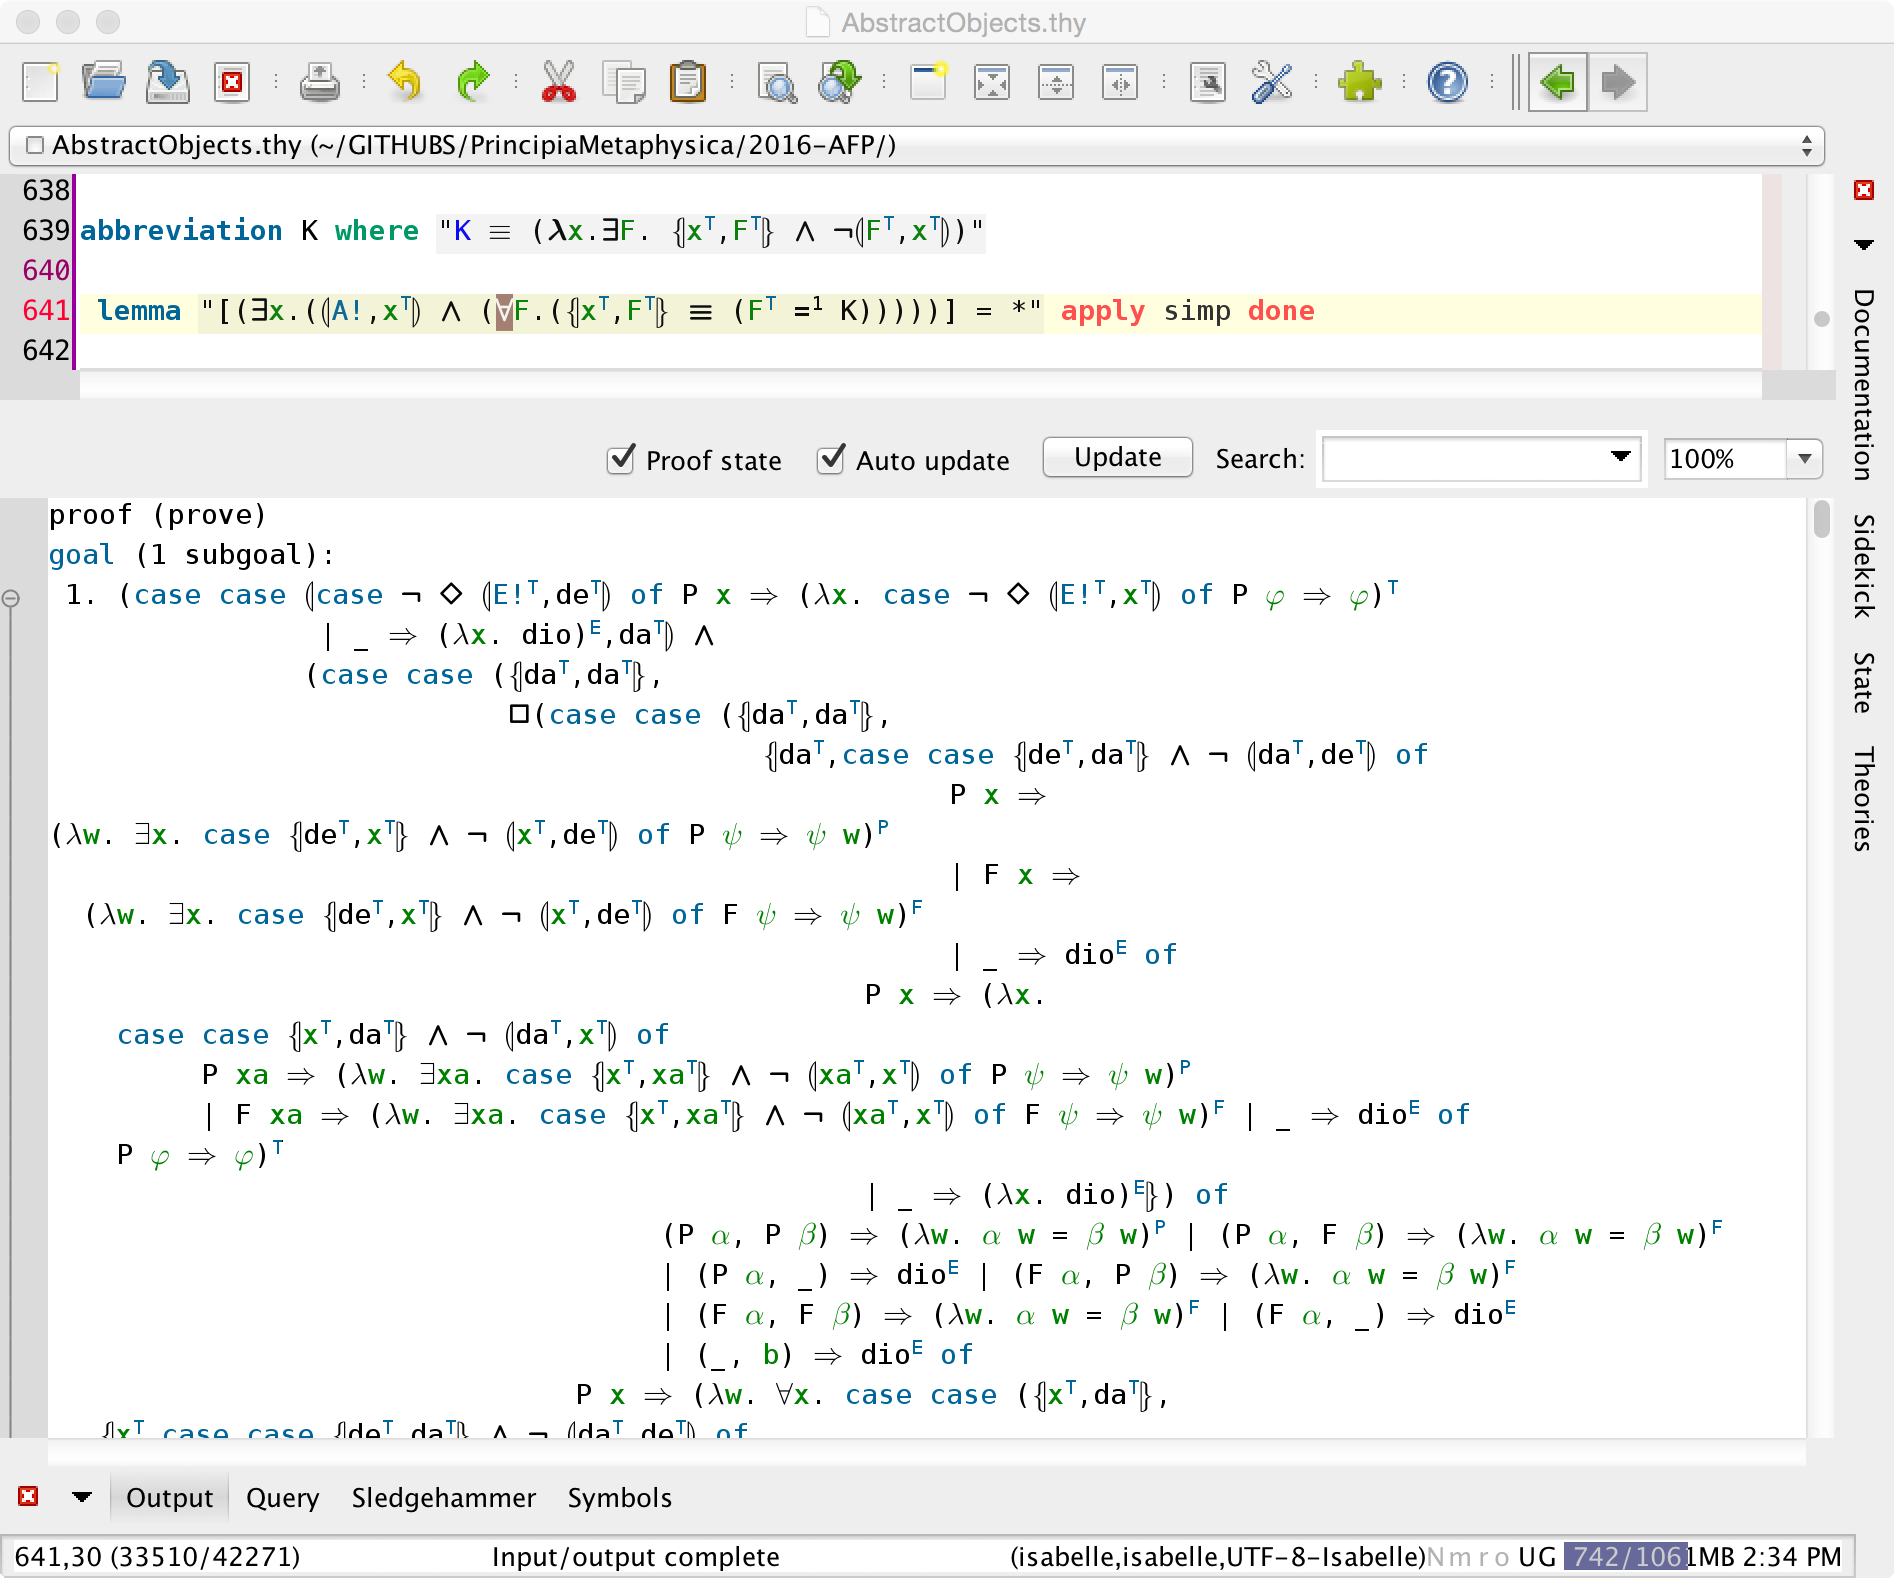
\includegraphics[width=.9\textwidth]{LargeTerm.png}
  \caption{Display (of about 5\%) of the unfolded expression \isa{{\isacharbrackleft}{\isacharparenleft}\isactrlbold {\isasymexists}x{\isachardot}{\isacharparenleft}{\isasymlparr}A{\isacharbang}{\isacharcomma}x\isactrlsup T{\isasymrparr}\ \isactrlbold {\isasymand}\ {\isacharparenleft}\isactrlbold {\isasymforall}F{\isachardot}\ {\isacharparenleft}{\isasymlbrace}x\isactrlsup T{\isacharcomma}F\isactrlsup T{\isasymrbrace}\ \isactrlbold {\isasymequiv}\ {\isacharparenleft}F\isactrlsup T\ \isactrlbold {\isacharequal}\isactrlsup {\isadigit{1}}\ K{\isacharparenright}{\isacharparenright}{\isacharparenright}{\isacharparenright}{\isacharparenright}{\isacharbrackright}\ {\isacharequal}\ {\isacharasterisk}} 
 in Isabelle/HOL. \label{large}} 
  \end{figure}%
\end{isamarkuptext}%
\isamarkuptrue%
%
\isamarkupsection{Some Further Tests%
}
\isamarkuptrue%
%
\begin{isamarkuptext}%
In this section we present some further test examples of our encoding. Many of these tests are taken
 from papers (e.g. cf.~\cite{zalta11:_relat_versus_funct_found_logic} or presentation slides of Zalta.%
\end{isamarkuptext}%
\isamarkuptrue%
%
\begin{isamarkuptext}%
We show that the derivation from \isa{{\isacharparenleft}{\isasymlbrace}a\isactrlsup T{\isacharcomma}PP\isactrlsup T{\isasymrbrace}\ \isactrlbold {\isasymand}\ \isactrlbold {\isasymnot}{\isasymlparr}PP\isactrlsup T{\isacharcomma}a\isactrlsup T{\isasymrparr}{\isacharparenright}} 
to \isa{{\isacharparenleft}\isactrlbold {\isasymexists}F{\isachardot}{\isasymlbrace}a\isactrlsup T{\isacharcomma}F\isactrlsup T{\isasymrbrace}\ \isactrlbold {\isasymand}\ \isactrlbold {\isasymnot}{\isasymlparr}F\isactrlsup T{\isacharcomma}a\isactrlsup T{\isasymrparr}{\isacharparenright}} can in fact be 
represented and solved in our approach, 
cf. ~\cite[chap.4]{zalta11:_relat_versus_funct_found_logic}%
\end{isamarkuptext}%
\isamarkuptrue%
\ \isacommand{lemma}\isamarkupfalse%
\ {\isachardoublequoteopen}{\isacharbrackleft}{\isacharparenleft}{\isasymlbrace}a\isactrlsup T{\isacharcomma}PP\isactrlsup T{\isasymrbrace}\ \isactrlbold {\isasymand}\ \isactrlbold {\isasymnot}{\isasymlparr}PP\isactrlsup T{\isacharcomma}a\isactrlsup T{\isasymrparr}{\isacharparenright}{\isacharbrackright}\ {\isacharequal}\ {\isasymtop}\ {\isasymlongrightarrow}\ {\isacharbrackleft}{\isacharparenleft}\isactrlbold {\isasymexists}F{\isachardot}{\isasymlbrace}a\isactrlsup T{\isacharcomma}F\isactrlsup T{\isasymrbrace}\ \isactrlbold {\isasymand}\ \isactrlbold {\isasymnot}{\isasymlparr}F\isactrlsup T{\isacharcomma}a\isactrlsup T{\isasymrparr}{\isacharparenright}{\isacharbrackright}\ {\isacharequal}\ {\isasymtop}{\isachardoublequoteclose}%
\isadelimproof
\ %
\endisadelimproof
%
\isatagproof
\isacommand{apply}\isamarkupfalse%
\ simp\ \isacommand{by}\isamarkupfalse%
\ auto%
\endisatagproof
{\isafoldproof}%
%
\isadelimproof
%
\endisadelimproof
%
\isamarkupsubsection{Properties of Equality%
}
\isamarkuptrue%
\ \isacommand{lemma}\isamarkupfalse%
\ {\isachardoublequoteopen}{\isacharbrackleft}{\isacharparenleft}\isactrlbold {\isasymforall}x{\isachardot}\ {\isasymlparr}O{\isacharbang}{\isacharcomma}x\isactrlsup T{\isasymrparr}\ \isactrlbold {\isasymrightarrow}\ x\isactrlsup T\ \isactrlbold {\isacharequal}\ x\isactrlsup T{\isacharparenright}{\isacharbrackright}\ {\isacharequal}\ {\isasymtop}{\isachardoublequoteclose}%
\isadelimproof
\ %
\endisadelimproof
%
\isatagproof
\isacommand{apply}\isamarkupfalse%
\ simp\ \isacommand{done}\isamarkupfalse%
%
\endisatagproof
{\isafoldproof}%
%
\isadelimproof
%
\endisadelimproof
\isanewline
\ \isacommand{lemma}\isamarkupfalse%
\ {\isachardoublequoteopen}{\isacharbrackleft}{\isacharparenleft}\isactrlbold {\isasymforall}x{\isachardot}\ {\isasymlparr}A{\isacharbang}{\isacharcomma}x\isactrlsup T{\isasymrparr}\ \isactrlbold {\isasymrightarrow}\ x\isactrlsup T\ \isactrlbold {\isacharequal}\ x\isactrlsup T{\isacharparenright}{\isacharbrackright}\ {\isacharequal}\ {\isasymtop}{\isachardoublequoteclose}%
\isadelimproof
\ %
\endisadelimproof
%
\isatagproof
\isacommand{apply}\isamarkupfalse%
\ simp\ \isacommand{done}\isamarkupfalse%
%
\endisatagproof
{\isafoldproof}%
%
\isadelimproof
%
\endisadelimproof
\isanewline
\ \isacommand{lemma}\isamarkupfalse%
\ {\isachardoublequoteopen}{\isacharbrackleft}{\isacharparenleft}\isactrlbold {\isasymforall}x\ y{\isachardot}\ x\isactrlsup T\ \isactrlbold {\isacharequal}\ y\isactrlsup T\ \isactrlbold {\isasymrightarrow}\ y\isactrlsup T\ \isactrlbold {\isacharequal}\ x\isactrlsup T{\isacharparenright}{\isacharbrackright}\ {\isacharequal}\ {\isasymtop}{\isachardoublequoteclose}%
\isadelimproof
\ %
\endisadelimproof
%
\isatagproof
\isacommand{apply}\isamarkupfalse%
\ simp\ \isacommand{by}\isamarkupfalse%
\ meson%
\endisatagproof
{\isafoldproof}%
%
\isadelimproof
%
\endisadelimproof
\isanewline
\ \isacommand{lemma}\isamarkupfalse%
\ {\isachardoublequoteopen}{\isacharbrackleft}{\isacharparenleft}\isactrlbold {\isasymforall}x\ y\ z{\isachardot}\ {\isacharparenleft}x\isactrlsup T\ \isactrlbold {\isacharequal}\ y\isactrlsup T\ \isactrlbold {\isasymand}\ y\isactrlsup T\ \isactrlbold {\isacharequal}\ z\isactrlsup T{\isacharparenright}\ \isactrlbold {\isasymrightarrow}\ x\isactrlsup T\ \isactrlbold {\isacharequal}\ z\isactrlsup T{\isacharparenright}{\isacharbrackright}\ {\isacharequal}\ {\isasymtop}{\isachardoublequoteclose}%
\isadelimproof
\ %
\endisadelimproof
%
\isatagproof
\isacommand{apply}\isamarkupfalse%
\ simp\ \isacommand{by}\isamarkupfalse%
\ meson%
\endisatagproof
{\isafoldproof}%
%
\isadelimproof
%
\endisadelimproof
\isanewline
\isanewline
\isanewline
\isanewline
\isanewline
\ \isacommand{lemma}\isamarkupfalse%
\ {\isachardoublequoteopen}{\isacharbrackleft}{\isacharparenleft}\isactrlbold {\isasymforall}x{\isachardot}\ {\isasymlparr}O{\isacharbang}{\isacharcomma}x\isactrlsup T{\isasymrparr}\ \isactrlbold {\isasymrightarrow}\ x\isactrlsup T\ \isactrlbold {\isacharequal}\isactrlsub E\ x\isactrlsup T{\isacharparenright}{\isacharbrackright}\ {\isacharequal}\ {\isasymtop}{\isachardoublequoteclose}%
\isadelimproof
\ %
\endisadelimproof
%
\isatagproof
\isacommand{apply}\isamarkupfalse%
\ simp\ \isacommand{done}\isamarkupfalse%
%
\endisatagproof
{\isafoldproof}%
%
\isadelimproof
%
\endisadelimproof
\isanewline
\ \isacommand{lemma}\isamarkupfalse%
\ {\isachardoublequoteopen}{\isacharbrackleft}{\isacharparenleft}\isactrlbold {\isasymforall}x\ y{\isachardot}\ x\isactrlsup T\ \isactrlbold {\isacharequal}\isactrlsub E\ y\isactrlsup T\ \isactrlbold {\isasymrightarrow}\ y\isactrlsup T\ \isactrlbold {\isacharequal}\isactrlsub E\ x\isactrlsup T{\isacharparenright}{\isacharbrackright}\ {\isacharequal}\ {\isasymtop}{\isachardoublequoteclose}%
\isadelimproof
\ %
\endisadelimproof
%
\isatagproof
\isacommand{apply}\isamarkupfalse%
\ simp\ \isacommand{done}\isamarkupfalse%
%
\endisatagproof
{\isafoldproof}%
%
\isadelimproof
%
\endisadelimproof
\isanewline
\ \isacommand{lemma}\isamarkupfalse%
\ {\isachardoublequoteopen}{\isacharbrackleft}{\isacharparenleft}\isactrlbold {\isasymforall}x\ y\ z{\isachardot}\ {\isacharparenleft}x\isactrlsup T\ \isactrlbold {\isacharequal}\isactrlsub E\ y\isactrlsup T\ \isactrlbold {\isasymand}\ y\isactrlsup T\ \isactrlbold {\isacharequal}\isactrlsub E\ z\isactrlsup T{\isacharparenright}\ \isactrlbold {\isasymrightarrow}\ x\isactrlsup T\ \isactrlbold {\isacharequal}\isactrlsub E\ z\isactrlsup T{\isacharparenright}{\isacharbrackright}\ {\isacharequal}\ {\isasymtop}{\isachardoublequoteclose}%
\isadelimproof
\ %
\endisadelimproof
%
\isatagproof
\isacommand{apply}\isamarkupfalse%
\ simp\ \isacommand{done}\isamarkupfalse%
%
\endisatagproof
{\isafoldproof}%
%
\isadelimproof
%
\endisadelimproof
\isanewline
\isanewline
\isanewline
\ \isacommand{lemma}\isamarkupfalse%
\ {\isachardoublequoteopen}{\isacharbrackleft}{\isacharparenleft}\isactrlbold {\isasymforall}x{\isachardot}\ x\isactrlsup P\ \isactrlbold {\isacharequal}\isactrlsup {\isadigit{0}}\ x\isactrlsup P{\isacharparenright}{\isacharbrackright}\ {\isacharequal}\ {\isasymtop}{\isachardoublequoteclose}%
\isadelimproof
\ %
\endisadelimproof
%
\isatagproof
\isacommand{apply}\isamarkupfalse%
\ simp\ \isacommand{done}\isamarkupfalse%
%
\endisatagproof
{\isafoldproof}%
%
\isadelimproof
%
\endisadelimproof
\isanewline
\ \isacommand{lemma}\isamarkupfalse%
\ {\isachardoublequoteopen}{\isacharbrackleft}{\isacharparenleft}\isactrlbold {\isasymforall}x\ y{\isachardot}\ x\isactrlsup P\ \isactrlbold {\isacharequal}\isactrlsup {\isadigit{0}}\ y\isactrlsup P\ \isactrlbold {\isasymrightarrow}\ y\isactrlsup P\ \isactrlbold {\isacharequal}\isactrlsup {\isadigit{0}}\ x\isactrlsup P{\isacharparenright}{\isacharbrackright}\ {\isacharequal}\ {\isasymtop}{\isachardoublequoteclose}%
\isadelimproof
\ %
\endisadelimproof
%
\isatagproof
\isacommand{apply}\isamarkupfalse%
\ simp\ \isacommand{done}\isamarkupfalse%
%
\endisatagproof
{\isafoldproof}%
%
\isadelimproof
%
\endisadelimproof
\isanewline
\ \isacommand{lemma}\isamarkupfalse%
\ {\isachardoublequoteopen}{\isacharbrackleft}{\isacharparenleft}\isactrlbold {\isasymforall}x\ y\ z{\isachardot}\ {\isacharparenleft}x\isactrlsup P\ \isactrlbold {\isacharequal}\isactrlsup {\isadigit{0}}\ y\isactrlsup P\ \isactrlbold {\isasymand}\ y\isactrlsup P\ \isactrlbold {\isacharequal}\isactrlsup {\isadigit{0}}\ z\isactrlsup P{\isacharparenright}\ \isactrlbold {\isasymrightarrow}\ x\isactrlsup P\ \isactrlbold {\isacharequal}\isactrlsup {\isadigit{0}}\ z\isactrlsup P{\isacharparenright}{\isacharbrackright}\ {\isacharequal}\ {\isasymtop}{\isachardoublequoteclose}%
\isadelimproof
\ %
\endisadelimproof
%
\isatagproof
\isacommand{apply}\isamarkupfalse%
\ simp\ \isacommand{done}\isamarkupfalse%
%
\endisatagproof
{\isafoldproof}%
%
\isadelimproof
%
\endisadelimproof
\isanewline
\isanewline
\isanewline
\ \isacommand{lemma}\isamarkupfalse%
\ {\isachardoublequoteopen}{\isacharbrackleft}{\isacharparenleft}\isactrlbold {\isasymforall}x{\isachardot}\ x\isactrlsup P\ \isactrlbold {\isacharequal}\isactrlsup {\isadigit{0}}\ x\isactrlsup P{\isacharparenright}{\isacharbrackright}\ {\isacharequal}\ {\isasymtop}{\isachardoublequoteclose}%
\isadelimproof
\ %
\endisadelimproof
%
\isatagproof
\isacommand{apply}\isamarkupfalse%
\ simp\ \isacommand{done}\isamarkupfalse%
%
\endisatagproof
{\isafoldproof}%
%
\isadelimproof
%
\endisadelimproof
\isanewline
\ \isacommand{lemma}\isamarkupfalse%
\ {\isachardoublequoteopen}{\isacharbrackleft}{\isacharparenleft}\isactrlbold {\isasymforall}x\ y{\isachardot}\ x\isactrlsup P\ \isactrlbold {\isacharequal}\isactrlsup {\isadigit{0}}\ y\isactrlsup P\ \isactrlbold {\isasymrightarrow}\ y\isactrlsup P\ \isactrlbold {\isacharequal}\isactrlsup {\isadigit{0}}\ x\isactrlsup P{\isacharparenright}{\isacharbrackright}\ {\isacharequal}\ {\isasymtop}{\isachardoublequoteclose}%
\isadelimproof
\ %
\endisadelimproof
%
\isatagproof
\isacommand{apply}\isamarkupfalse%
\ simp\ \isacommand{done}\isamarkupfalse%
%
\endisatagproof
{\isafoldproof}%
%
\isadelimproof
%
\endisadelimproof
\isanewline
\ \isacommand{lemma}\isamarkupfalse%
\ {\isachardoublequoteopen}{\isacharbrackleft}{\isacharparenleft}\isactrlbold {\isasymforall}x\ y\ z{\isachardot}\ {\isacharparenleft}x\isactrlsup P\ \isactrlbold {\isacharequal}\isactrlsup {\isadigit{0}}\ y\isactrlsup P\ \isactrlbold {\isasymand}\ y\isactrlsup P\ \isactrlbold {\isacharequal}\isactrlsup {\isadigit{0}}\ z\isactrlsup P{\isacharparenright}\ \isactrlbold {\isasymrightarrow}\ x\isactrlsup P\ \isactrlbold {\isacharequal}\isactrlsup {\isadigit{0}}\ z\isactrlsup P{\isacharparenright}{\isacharbrackright}\ {\isacharequal}\ {\isasymtop}{\isachardoublequoteclose}%
\isadelimproof
\ %
\endisadelimproof
%
\isatagproof
\isacommand{apply}\isamarkupfalse%
\ simp\ \isacommand{done}\isamarkupfalse%
%
\endisatagproof
{\isafoldproof}%
%
\isadelimproof
%
\endisadelimproof
\isanewline
\isanewline
\isanewline
\ \isacommand{lemma}\isamarkupfalse%
\ {\isachardoublequoteopen}{\isacharbrackleft}{\isacharparenleft}\isactrlbold {\isasymforall}x{\isachardot}\ x\isactrlsup T\ \isactrlbold {\isacharequal}\isactrlsup {\isadigit{1}}\ x\isactrlsup T{\isacharparenright}{\isacharbrackright}\ {\isacharequal}\ {\isasymtop}{\isachardoublequoteclose}%
\isadelimproof
\ %
\endisadelimproof
%
\isatagproof
\isacommand{apply}\isamarkupfalse%
\ simp\ \isacommand{done}\isamarkupfalse%
%
\endisatagproof
{\isafoldproof}%
%
\isadelimproof
%
\endisadelimproof
\isanewline
\ \isacommand{lemma}\isamarkupfalse%
\ {\isachardoublequoteopen}{\isacharbrackleft}{\isacharparenleft}\isactrlbold {\isasymforall}x\ y{\isachardot}\ x\isactrlsup T\ \isactrlbold {\isacharequal}\isactrlsup {\isadigit{1}}\ y\isactrlsup T\ \isactrlbold {\isasymrightarrow}\ y\isactrlsup T\ \isactrlbold {\isacharequal}\isactrlsup {\isadigit{1}}\ x\isactrlsup T{\isacharparenright}{\isacharbrackright}\ {\isacharequal}\ {\isasymtop}{\isachardoublequoteclose}%
\isadelimproof
\ %
\endisadelimproof
%
\isatagproof
\isacommand{apply}\isamarkupfalse%
\ simp\ \isacommand{done}\isamarkupfalse%
%
\endisatagproof
{\isafoldproof}%
%
\isadelimproof
%
\endisadelimproof
\isanewline
\ \isacommand{lemma}\isamarkupfalse%
\ {\isachardoublequoteopen}{\isacharbrackleft}{\isacharparenleft}\isactrlbold {\isasymforall}x\ y\ z{\isachardot}\ {\isacharparenleft}x\isactrlsup T\ \isactrlbold {\isacharequal}\isactrlsup {\isadigit{1}}\ y\isactrlsup T\ \isactrlbold {\isasymand}\ y\isactrlsup T\ \isactrlbold {\isacharequal}\isactrlsup {\isadigit{1}}\ z\isactrlsup T{\isacharparenright}\ \isactrlbold {\isasymrightarrow}\ x\isactrlsup T\ \isactrlbold {\isacharequal}\isactrlsup {\isadigit{1}}\ z\isactrlsup T{\isacharparenright}{\isacharbrackright}\ {\isacharequal}\ {\isasymtop}{\isachardoublequoteclose}%
\isadelimproof
\ %
\endisadelimproof
%
\isatagproof
\isacommand{apply}\isamarkupfalse%
\ simp\ \isacommand{done}\isamarkupfalse%
%
\endisatagproof
{\isafoldproof}%
%
\isadelimproof
%
\endisadelimproof
\isanewline
\isanewline
\isanewline
\ \isacommand{lemma}\isamarkupfalse%
\ {\isachardoublequoteopen}{\isacharbrackleft}{\isacharparenleft}\isactrlbold {\isasymforall}x{\isachardot}\ x\isactrlsup T\ \isactrlbold {\isacharequal}\isactrlsup {\isadigit{2}}\ x\isactrlsup T{\isacharparenright}{\isacharbrackright}\ {\isacharequal}\ {\isasymtop}{\isachardoublequoteclose}%
\isadelimproof
\ %
\endisadelimproof
%
\isatagproof
\isacommand{apply}\isamarkupfalse%
\ simp\ \isacommand{done}\isamarkupfalse%
%
\endisatagproof
{\isafoldproof}%
%
\isadelimproof
%
\endisadelimproof
\isanewline
\ \isacommand{lemma}\isamarkupfalse%
\ {\isachardoublequoteopen}{\isacharbrackleft}{\isacharparenleft}\isactrlbold {\isasymforall}x\ y{\isachardot}\ x\isactrlsup T\ \isactrlbold {\isacharequal}\isactrlsup {\isadigit{2}}\ y\isactrlsup T\ \isactrlbold {\isasymrightarrow}\ y\isactrlsup T\ \isactrlbold {\isacharequal}\isactrlsup {\isadigit{2}}\ x\isactrlsup T{\isacharparenright}{\isacharbrackright}\ {\isacharequal}\ {\isasymtop}{\isachardoublequoteclose}%
\isadelimproof
\ %
\endisadelimproof
%
\isatagproof
\isacommand{apply}\isamarkupfalse%
\ simp\ \isacommand{done}\isamarkupfalse%
%
\endisatagproof
{\isafoldproof}%
%
\isadelimproof
%
\endisadelimproof
\isanewline
\ \isacommand{lemma}\isamarkupfalse%
\ {\isachardoublequoteopen}{\isacharbrackleft}{\isacharparenleft}\isactrlbold {\isasymforall}x\ y\ z{\isachardot}\ {\isacharparenleft}x\isactrlsup T\ \isactrlbold {\isacharequal}\isactrlsup {\isadigit{2}}\ y\isactrlsup T\ \isactrlbold {\isasymand}\ y\isactrlsup T\ \isactrlbold {\isacharequal}\isactrlsup {\isadigit{2}}\ z\isactrlsup T{\isacharparenright}\ \isactrlbold {\isasymrightarrow}\ x\isactrlsup T\ \isactrlbold {\isacharequal}\isactrlsup {\isadigit{2}}\ z\isactrlsup T{\isacharparenright}{\isacharbrackright}\ {\isacharequal}\ {\isasymtop}{\isachardoublequoteclose}%
\isadelimproof
\ %
\endisadelimproof
%
\isatagproof
\isacommand{apply}\isamarkupfalse%
\ simp\ \isacommand{done}\isamarkupfalse%
%
\endisatagproof
{\isafoldproof}%
%
\isadelimproof
%
\endisadelimproof
\isanewline
\isanewline
\isanewline
\ \isacommand{lemma}\isamarkupfalse%
\ {\isachardoublequoteopen}{\isacharbrackleft}{\isacharparenleft}\isactrlbold {\isasymforall}x{\isachardot}\ x\isactrlsup T\ \isactrlbold {\isacharequal}\isactrlsup {\isadigit{3}}\ x\isactrlsup T{\isacharparenright}{\isacharbrackright}\ {\isacharequal}\ {\isasymtop}{\isachardoublequoteclose}%
\isadelimproof
\ %
\endisadelimproof
%
\isatagproof
\isacommand{apply}\isamarkupfalse%
\ simp\ \isacommand{done}\isamarkupfalse%
%
\endisatagproof
{\isafoldproof}%
%
\isadelimproof
%
\endisadelimproof
\isanewline
\ \isacommand{lemma}\isamarkupfalse%
\ {\isachardoublequoteopen}{\isacharbrackleft}{\isacharparenleft}\isactrlbold {\isasymforall}x\ y{\isachardot}\ x\isactrlsup T\ \isactrlbold {\isacharequal}\isactrlsup {\isadigit{3}}\ y\isactrlsup T\ \isactrlbold {\isasymrightarrow}\ y\isactrlsup T\ \isactrlbold {\isacharequal}\isactrlsup {\isadigit{3}}\ x\isactrlsup T{\isacharparenright}{\isacharbrackright}\ {\isacharequal}\ {\isasymtop}{\isachardoublequoteclose}%
\isadelimproof
\ %
\endisadelimproof
%
\isatagproof
\isacommand{apply}\isamarkupfalse%
\ simp\ \isacommand{done}\isamarkupfalse%
%
\endisatagproof
{\isafoldproof}%
%
\isadelimproof
%
\endisadelimproof
\isanewline
\ \isacommand{lemma}\isamarkupfalse%
\ {\isachardoublequoteopen}{\isacharbrackleft}{\isacharparenleft}\isactrlbold {\isasymforall}x\ y\ z{\isachardot}\ {\isacharparenleft}x\isactrlsup T\ \isactrlbold {\isacharequal}\isactrlsup {\isadigit{3}}\ y\isactrlsup T\ \isactrlbold {\isasymand}\ y\isactrlsup T\ \isactrlbold {\isacharequal}\isactrlsup {\isadigit{3}}\ z\isactrlsup T{\isacharparenright}\ \isactrlbold {\isasymrightarrow}\ x\isactrlsup T\ \isactrlbold {\isacharequal}\isactrlsup {\isadigit{3}}\ z\isactrlsup T{\isacharparenright}{\isacharbrackright}\ {\isacharequal}\ {\isasymtop}{\isachardoublequoteclose}%
\isadelimproof
\ %
\endisadelimproof
%
\isatagproof
\isacommand{apply}\isamarkupfalse%
\ simp\ \isacommand{done}\isamarkupfalse%
%
\endisatagproof
{\isafoldproof}%
%
\isadelimproof
%
\endisadelimproof
%
\isamarkupsubsection{Technological problem/Pushing Isabelle to its Limits%
}
\isamarkuptrue%
%
\begin{isamarkuptext}%
While the latter formulas can still be verified by simp, 
  their unfolded internal representations cannot be displayed anymore in Isabelle/HOL's jedit based
  user interface on a
  standard Macbook. Isabelle in fact reports the following: 
     ``No subgoals! exception Size raised (line 182 of "./basis/LibrarySupport.sml")''
  Displaying the internal unfolded representation still worked 
  for \isa{{\isacharbrackleft}{\isacharparenleft}\isactrlbold {\isasymforall}x\ y{\isachardot}\ x\isactrlsup T\ \isactrlbold {\isacharequal}\isactrlsup {\isadigit{3}}\ y\isactrlsup T\ \isactrlbold {\isasymrightarrow}\ y\isactrlsup T\ \isactrlbold {\isacharequal}\isactrlsup {\isadigit{3}}\ x\isactrlsup T{\isacharparenright}{\isacharbrackright}\ {\isacharequal}\ {\isasymtop}} though. This term is presented in the appendix 
  of this paper (on about 240 pages in scriptsize).%
\end{isamarkuptext}%
\isamarkuptrue%
%
\isamarkupsubsection{Axioms and Tests for Actuality%
}
\isamarkuptrue%
%
\begin{isamarkuptext}%
One issue that we did not address yet is how one can possibly encode 
 axiom schemata like \isa{\isactrlbold {\isasymA}{\isasymphi}\ \isactrlbold {\isasymrightarrow}\ \isactrlbold {\isasymphi}} where \isa{\isactrlbold {\isasymphi}} ranges only 
 over \isa{\isactrlbold {\isasymbox}}-free closures. Eventually the grammar should be further refined so that we get a 
 category of \isa{\isactrlbold {\isasymbox}}-free formulas?%
\end{isamarkuptext}%
\isamarkuptrue%
\ \isacommand{lemma}\isamarkupfalse%
\ {\isachardoublequoteopen}{\isacharbrackleft}\isactrlbold {\isasymA}{\isasymphi}\isactrlsup P\ \isactrlbold {\isasymrightarrow}\ \isactrlbold {\isasymbox}{\isacharparenleft}\isactrlbold {\isasymA}{\isasymphi}\isactrlsup P{\isacharparenright}{\isacharbrackright}\ {\isacharequal}\ {\isasymtop}{\isachardoublequoteclose}%
\isadelimproof
\ %
\endisadelimproof
%
\isatagproof
\isacommand{apply}\isamarkupfalse%
\ simp\ \isacommand{done}\isamarkupfalse%
%
\endisatagproof
{\isafoldproof}%
%
\isadelimproof
%
\endisadelimproof
\isanewline
\ \isacommand{lemma}\isamarkupfalse%
\ {\isachardoublequoteopen}{\isacharbrackleft}\isactrlbold {\isasymA}{\isasymphi}\isactrlsup F\ \isactrlbold {\isasymrightarrow}\ \isactrlbold {\isasymbox}{\isacharparenleft}\isactrlbold {\isasymA}{\isasymphi}\isactrlsup F{\isacharparenright}{\isacharbrackright}\ {\isacharequal}\ {\isasymtop}{\isachardoublequoteclose}%
\isadelimproof
\ %
\endisadelimproof
%
\isatagproof
\isacommand{apply}\isamarkupfalse%
\ simp\ \isacommand{done}\isamarkupfalse%
%
\endisatagproof
{\isafoldproof}%
%
\isadelimproof
%
\endisadelimproof
%
\isamarkupsubsection{Theory of Encoding%
}
\isamarkuptrue%
%
\begin{isamarkuptext}%
We present a small case study in the theory of encoding. For this we first
 postulate some axioms and provide some further definitions/abbreviations.%
\end{isamarkuptext}%
\isamarkuptrue%
\ \isacommand{axiomatization}\isamarkupfalse%
\ \isakeyword{where}\isanewline
\ \ RigityOfEncoding{\isacharcolon}\ \ {\isachardoublequoteopen}{\isacharbrackleft}{\isasymlbrace}x\isactrlsup T{\isacharcomma}FF\isactrlsup T{\isasymrbrace}\ \isactrlbold {\isasymrightarrow}\ \isactrlbold {\isasymbox}{\isasymlbrace}x\isactrlsup T{\isacharcomma}FF\isactrlsup T{\isasymrbrace}{\isacharbrackright}\ {\isacharequal}\ {\isasymtop}{\isachardoublequoteclose}\ \isakeyword{and}\isanewline
\ \ OrdinaryObjectsDoNotEncode{\isacharcolon}\ {\isachardoublequoteopen}{\isacharbrackleft}{\isasymlparr}O{\isacharbang}{\isacharcomma}x\isactrlsup T{\isasymrparr}\ \isactrlbold {\isasymrightarrow}\ \isactrlbold {\isasymbox}{\isacharparenleft}\isactrlbold {\isasymnot}{\isacharparenleft}\isactrlbold {\isasymexists}F{\isachardot}\ {\isasymlbrace}x\isactrlsup T{\isacharcomma}F\isactrlsup T{\isasymrbrace}{\isacharparenright}{\isacharparenright}{\isacharbrackright}\ {\isacharequal}\ {\isasymtop}{\isachardoublequoteclose}\ \isakeyword{and}\isanewline
\ \ ObjectComprehension{\isacharcolon}\ {\isachardoublequoteopen}{\isacharbrackleft}{\isacharparenleft}\isactrlbold {\isasymexists}x{\isachardot}\ {\isasymlparr}A{\isacharbang}{\isacharcomma}x\isactrlsup T{\isasymrparr}\ \isactrlbold {\isasymand}\ {\isacharparenleft}\isactrlbold {\isasymforall}F{\isachardot}\ {\isasymlbrace}x\isactrlsup T{\isacharcomma}F\isactrlsup T{\isasymrbrace}\ \isactrlbold {\isasymequiv}\ {\isasymphi}{\isacharparenright}{\isacharparenright}{\isacharbrackright}\ {\isacharequal}\ {\isasymtop}{\isachardoublequoteclose}\isanewline
\isanewline
\ \isacommand{abbreviation}\isamarkupfalse%
\ Situation{\isacharcolon}{\isacharcolon}{\isachardoublequoteopen}e\ opt{\isasymRightarrow}io\ opt{\isachardoublequoteclose}\ \ \isakeyword{where}\ \isanewline
\ \ \ {\isachardoublequoteopen}Situation\ x\ {\isasymequiv}\ {\isacharparenleft}{\isasymlparr}A{\isacharbang}{\isacharcomma}x{\isasymrparr}\ \isactrlbold {\isasymand}\ {\isacharparenleft}\isactrlbold {\isasymforall}F{\isachardot}\ {\isacharparenleft}{\isasymlbrace}x{\isacharcomma}F\isactrlsup T{\isasymrbrace}\ \isactrlbold {\isasymrightarrow}\ {\isacharparenleft}\isactrlbold {\isasymexists}p{\isachardot}\ F\isactrlsup T\ \isactrlbold {\isacharequal}\isactrlsup {\isadigit{1}}\ {\isacharparenleft}\isactrlbold {\isasymlambda}y{\isachardot}\ p\isactrlsup P{\isacharparenright}{\isacharparenright}{\isacharparenright}{\isacharparenright}{\isacharparenright}{\isachardoublequoteclose}\isanewline
\ \isacommand{abbreviation}\isamarkupfalse%
\ PIsTrueInX{\isacharcolon}{\isacharcolon}{\isachardoublequoteopen}e\ opt\ {\isasymRightarrow}\ {\isacharparenleft}i\ {\isasymRightarrow}\ bool{\isacharparenright}\ opt\ {\isasymRightarrow}\ {\isacharparenleft}i\ {\isasymRightarrow}\ bool{\isacharparenright}\ opt{\isachardoublequoteclose}\ {\isacharparenleft}\isakeyword{infixl}\ {\isachardoublequoteopen}{\isasymTurnstile}{\isachardoublequoteclose}\ {\isadigit{6}}{\isadigit{3}}{\isacharparenright}\ \isakeyword{where}\ \isanewline
\ \ \ {\isachardoublequoteopen}x\ {\isasymTurnstile}\ p\ {\isasymequiv}\ {\isasymlbrace}x{\isacharcomma}{\isacharparenleft}\isactrlbold {\isasymlambda}y{\isachardot}\ p{\isacharparenright}{\isasymrbrace}{\isachardoublequoteclose}\ \ \isanewline
\ \isacommand{abbreviation}\isamarkupfalse%
\ PossibleWorld{\isacharcolon}{\isacharcolon}{\isachardoublequoteopen}e\ opt{\isasymRightarrow}io\ opt{\isachardoublequoteclose}\ \isakeyword{where}\ \isanewline
\ \ \ {\isachardoublequoteopen}PossibleWorld\ x\ {\isasymequiv}\ Situation{\isacharparenleft}x{\isacharparenright}\ \isactrlbold {\isasymand}\ \isactrlbold {\isasymdiamond}{\isacharparenleft}\isactrlbold {\isasymforall}p{\isachardot}\ {\isacharparenleft}x\ {\isasymTurnstile}\ p\isactrlsup P{\isacharparenright}\ \isactrlbold {\isasymequiv}\ p\isactrlsup P{\isacharparenright}{\isachardoublequoteclose}\ \isanewline
\ \isacommand{abbreviation}\isamarkupfalse%
\ Maximal{\isacharcolon}{\isacharcolon}{\isachardoublequoteopen}e\ opt{\isasymRightarrow}io\ opt{\isachardoublequoteclose}\ \isakeyword{where}\ \isanewline
\ \ \ {\isachardoublequoteopen}Maximal\ s\ {\isasymequiv}\ {\isacharparenleft}\isactrlbold {\isasymforall}p{\isachardot}\ {\isacharparenleft}s\ {\isasymTurnstile}\ p\isactrlsup P{\isacharparenright}\ \isactrlbold {\isasymor}\ {\isacharparenleft}s\ {\isasymTurnstile}\ {\isacharparenleft}\isactrlbold {\isasymnot}\ p\isactrlsup P{\isacharparenright}{\isacharparenright}{\isacharparenright}{\isachardoublequoteclose}%
\begin{isamarkuptext}%
We are now in the position to formalize and prove the fundamental theorem of possible worlds,
  which states that possible worlds are maximal.%
\end{isamarkuptext}%
\isamarkuptrue%
\ \isacommand{lemma}\isamarkupfalse%
\ {\isachardoublequoteopen}{\isacharbrackleft}{\isacharparenleft}\isactrlbold {\isasymforall}x{\isachardot}\ PossibleWorld{\isacharparenleft}x\isactrlsup T{\isacharparenright}\ \isactrlbold {\isasymrightarrow}\ Maximal{\isacharparenleft}x\isactrlsup T{\isacharparenright}{\isacharparenright}{\isacharbrackright}\ {\isacharequal}\ {\isasymtop}{\isachardoublequoteclose}%
\isadelimproof
\ %
\endisadelimproof
%
\isatagproof
\isacommand{apply}\isamarkupfalse%
\ simp\ \isacommand{done}\isamarkupfalse%
%
\endisatagproof
{\isafoldproof}%
%
\isadelimproof
%
\endisadelimproof
%
\isamarkupsubsection{Consistency?%
}
\isamarkuptrue%
%
\begin{isamarkuptext}%
Unfortunately, neither Nitpick nor the available
  ATPs are capable of verifying or disproving the consistency of the introduced theory.%
\end{isamarkuptext}%
\isamarkuptrue%
\ \isacommand{lemma}\isamarkupfalse%
\ True\ \isacommand{nitpick}\isamarkupfalse%
\ {\isacharbrackleft}satisfy{\isacharcomma}\ user{\isacharunderscore}axioms{\isacharbrackright}%
\isadelimproof
\ %
\endisadelimproof
%
\isatagproof
\isacommand{oops}\isamarkupfalse%
%
\endisatagproof
{\isafoldproof}%
%
\isadelimproof
%
\endisadelimproof
\ \isanewline
\ \isacommand{lemma}\isamarkupfalse%
\ False\ \isacommand{sledgehammer}\isamarkupfalse%
\ {\isacharbrackleft}remote{\isacharunderscore}leo{\isadigit{2}}\ remote{\isacharunderscore}satallax{\isacharbrackright}%
\isadelimproof
\ %
\endisadelimproof
%
\isatagproof
\isacommand{oops}\isamarkupfalse%
%
\endisatagproof
{\isafoldproof}%
%
\isadelimproof
%
\endisadelimproof
\isanewline
\ \isacommand{lemma}\isamarkupfalse%
\ False\ \isacommand{sledgehammer}\isamarkupfalse%
%
\isadelimproof
\ %
\endisadelimproof
%
\isatagproof
\isacommand{oops}\isamarkupfalse%
%
\endisatagproof
{\isafoldproof}%
%
\isadelimproof
%
\endisadelimproof
%
\isamarkupsection{Conclusion%
}
\isamarkuptrue%
%
\begin{isamarkuptext}%
We have experimented with an new idea towards a shallow embedding of MRTT in 
  functional type theory 
  and we have pushed the technical 
  elaboration of that idea to some interesting intermediate state.   
  While our embedding is clearly infeasible for pen and paper methods, 
  our original hope has been that -- modulo our embedding -- interactive and automated theorem provers for 
  functional type theory could, at least to a reasonable extend, be (re-)used for reasoning within
  MRTT and subsequently for reasoning in the theory of abstract objects. 


  However, within the 
  system infrastructure of Isabelle/HOL we seem to reach some technological limits (e.g. the internal formula
  representing the transitivity of equality between ternary relations cannot be displayed anymore 
 because of its size and consistency can neither be proved nor disproved anymore, etc.).
 On the other hand, we were still able automatically confirm the 
 fundamental theorem of possible worlds, and in this respect the degree of automation provided in our
 experiments exceeds that of related previous work \cite{ZaltaCade}.

 Independent of the outcome of the further research based upon the presented embedding it should 
 become clear that building a system similar to Isabelle but with taking MRTT as its foundational 
 core logic (instead of functional type theory) would surely provide
 a technologically more appropriate base environment for the formalization and automation of the theory of abstract objects
 and the principia metaphysica.%
\end{isamarkuptext}%
\isamarkuptrue%
%
\isadelimtheory
%
\endisadelimtheory
%
\isatagtheory
%
\endisatagtheory
{\isafoldtheory}%
%
\isadelimtheory
\isanewline
%
\endisadelimtheory
\end{isabellebody}%
%%% Local Variables:
%%% mode: latex
%%% TeX-master: "root"
%%% End:
